\documentclass[12pt,a4paper]{report}
\usepackage[utf8]{inputenc}
\usepackage{graphicx}
\usepackage{enumitem}
\usepackage{hyperref}
\usepackage{amssymb}
\usepackage{xcolor}
\usepackage{geometry}
\usepackage{fancyhdr}
\usepackage{tcolorbox}
\usepackage{listings}
\usepackage{color}
\usepackage{multicol}
\usepackage{colortbl}
\usepackage{amsmath}
\usepackage{caption}
\usepackage{subcaption}
\usepackage{float}

\hypersetup{
	colorlinks=true,
	linkcolor=blue!70!black,
	citecolor=green!50!black,
	urlcolor=violet!70!black,
	pdftitle={Solving Poisson Equation with Point Singularities Using PINNs},
	pdfauthor={Your Name},
	pdfsubject={Physics-Informed Neural Networks},
	pdfkeywords={PINNs, Poisson Equation, DeepXDE, Singularities, PDE, Deep Learning},
	pdfcreator={LaTeX},
	pdfproducer={pdfLaTeX}
}

\definecolor{codegreen}{rgb}{0,0.6,0}
\definecolor{codegray}{rgb}{0.5,0.5,0.5}
\definecolor{codepurple}{rgb}{0.58,0,0.82}
\definecolor{backcolour}{rgb}{0.95,0.95,0.92}

\lstdefinestyle{mystyle}{
	backgroundcolor=\color{backcolour},
	commentstyle=\color{codegreen},
	keywordstyle=\color{magenta},
	numberstyle=\tiny\color{codegray},
	stringstyle=\color{codepurple},
	basicstyle=\ttfamily\small,
	breaklines=true,
	captionpos=b,
	keepspaces=true,
	numbers=left,
	numbersep=5pt,
	showspaces=false,
	showstringspaces=false,
	showtabs=false,
	tabsize=2
}

\lstset{
	language=python,
	style=mystyle
}

\geometry{margin=1in}
\pagestyle{fancy}
\fancyhf{}
\setlength{\headheight}{15pt}
\renewcommand{\headrulewidth}{0.4pt}
\renewcommand{\footrulewidth}{0.4pt}
\fancyhead[L]{Poisson PINNs}
\fancyhead[R]{\thepage}
\fancyfoot[C]{\today}

\begin{document}
	
	\begin{titlepage}
		\centering
		{\Huge \scshape Solving 2D Poisson Equation with Point Singularities Using PINNs \par}
		\vspace{2cm}
		{\Large \bfseries \itshape Prepared by:\\}
		{\large Your Name\\}
		\vspace{1cm}
		{\large \today\\}
		\vfill
		{\Large Department of Electrical Engineering\\Your Institution}
	\end{titlepage}
	
	\tableofcontents
	\newpage
	
	\chapter{Introduction}
	The objective of this project is to solve the two-dimensional Poisson equation involving point singularities using Physics-Informed Neural Networks (PINNs) \cite{raissi2019physics}. This problem is particularly challenging for traditional numerical methods due to the presence of singularities at charge locations. The Poisson equation is fundamental in electrostatics, describing the relationship between electric potential and charge density \cite{griffiths2017introduction}.
	
	Physics-Informed Neural Networks represent a novel approach to solving partial differential equations (PDEs) by embedding physical laws into neural networks \cite{jagtap2022deep}. Unlike traditional numerical methods such as finite difference or finite element methods, PINNs incorporate the differential equations directly into the loss function during training, enforcing physics-based constraints throughout the domain.
	
	\section{Problem Statement}
	In this project, we focus on the two-dimensional Poisson equation for electrostatics:
	\begin{equation}
		\nabla^2 \phi = -\frac{\rho}{\varepsilon_0}
	\end{equation}
	
	Where:
	\begin{itemize}
		\item $\phi$ is the electric potential
		\item $\rho$ is the charge density
		\item $\varepsilon_0$ is the permittivity of free space (scaled to 1.0 in our implementation)
		\item $\nabla^2 = \frac{\partial^2}{\partial x^2} + \frac{\partial^2}{\partial y^2}$ is the Laplacian operator in 2D
	\end{itemize}
	
	The domain is a square region $\Omega = [-1, 1] \times [-1, 1]$ with Dirichlet boundary conditions:
	\begin{equation}
		\phi = 0 \quad \text{on} \quad \partial\Omega
	\end{equation}
	
	\section{Key Challenges}
	The main challenges in this problem include:
	\begin{itemize}
		\item \textbf{Singularities}: Point charges create singularities at their locations, making traditional numerical methods unstable.
		\item \textbf{Steep Gradients}: The solution exhibits rapid changes near the charges, requiring high resolution.
		\item \textbf{Accuracy}: Achieving high accuracy throughout the domain, especially near singularities.
	\end{itemize}
	
	\section{Project Objectives}
	The objectives of this project are:
	\begin{enumerate}
		\item Implement a PINN to solve the 2D Poisson equation with point charge singularities.
		\item Compare the PINN solution with the analytical solution.
		\item Visualize the electric potential and electric field.
		\item Analyze the performance of different network architectures and training strategies.
		\item Develop advanced visualization techniques for electric field and potential.
	\end{enumerate}
	
	\chapter{Theoretical Background}
	
	\section{The Poisson Equation in Electrostatics}
	The Poisson equation is a fundamental equation in many areas of physics, particularly in electrostatics \cite{evans2010partial}. In electrostatics, it relates the electric potential $\phi$ to the charge density $\rho$:
	
	\begin{equation}
		\nabla^2 \phi = -\frac{\rho}{\varepsilon_0}
	\end{equation}
	
	For point charges, the charge density is represented by Dirac delta functions:
	
	\begin{equation}
		\rho(\mathbf{r}) = \sum_{i} q_i \delta(\mathbf{r} - \mathbf{r}_i)
	\end{equation}
	
	Where $q_i$ is the magnitude of the $i$-th charge located at position $\mathbf{r}_i$.
	
	\section{Analytical Solution}
	For a 2D domain with point charges, the analytical solution to the Poisson equation is:
	
	\begin{equation}
		\phi(\mathbf{r}) = \sum_{i} \frac{q_i}{2\pi\varepsilon_0} \ln\left(\frac{1}{|\mathbf{r} - \mathbf{r}_i|}\right) + \phi_0
	\end{equation}
	
	Where $\phi_0$ is determined by the boundary conditions. In our case, with Dirichlet boundary conditions $\phi = 0$ on the boundary, $\phi_0$ must be chosen accordingly.
	
	This solution has logarithmic singularities at the charge locations, making it challenging for traditional numerical methods.
	
	\section{Physics-Informed Neural Networks (PINNs)}
	Physics-Informed Neural Networks (PINNs) are a class of neural networks that embed physical laws into the training process \cite{raissi2019physics, wang2020understanding}. The key concept is to incorporate the residual of the PDE into the loss function:
	
	\begin{equation}
		\mathcal{L}_{\text{PDE}} = \frac{1}{N_f} \sum_{i=1}^{N_f} \left| \nabla^2 \phi(\mathbf{x}_i) + \frac{\rho(\mathbf{x}_i)}{\varepsilon_0} \right|^2
	\end{equation}
	
	Where $\mathbf{x}_i$ are collocation points in the domain. Additionally, to enforce the boundary conditions:
	
	\begin{equation}
		\mathcal{L}_{\text{BC}} = \frac{1}{N_b} \sum_{i=1}^{N_b} \left| \phi(\mathbf{x}_i^b) - g(\mathbf{x}_i^b) \right|^2
	\end{equation}
	
	Where $\mathbf{x}_i^b$ are points on the boundary, and $g(\mathbf{x})$ is the prescribed boundary value (zero in our case).
	
	The total loss function is:
	
	\begin{equation}
		\mathcal{L} = \mathcal{L}_{\text{PDE}} + \lambda \mathcal{L}_{\text{BC}}
	\end{equation}
	
	Where $\lambda$ is a weighting factor.
	
	\section{Approximating Delta Functions}
	For numerical implementation, we approximate the Dirac delta function using a Gaussian function:
	
	\begin{equation}
		\delta(\mathbf{r}) \approx \frac{1}{2\pi\sigma^2} \exp\left(-\frac{|\mathbf{r}|^2}{2\sigma^2}\right)
	\end{equation}
	
	Where $\sigma$ is a small parameter controlling the width of the approximation. This smoothed representation helps in numerical stability while preserving the essential physics.
	
	\chapter{Methodology}
	
	\section{Problem Setup}
	We consider a 2D domain $\Omega = [-1, 1] \times [-1, 1]$ with two point charges:
	\begin{itemize}
		\item A positive charge with magnitude $q_1 = 1.0$ at position $(-0.5, 0.0)$
		\item A negative charge with magnitude $q_2 = -1.0$ at position $(0.5, 0.0)$
	\end{itemize}
	
	This configuration represents a simple electric dipole. We impose Dirichlet boundary conditions with $\phi = 0$ on all boundaries.
	
	\section{PINN Architecture}
	We use a fully connected neural network with the following architecture \cite{lu2021deepxde, goodfellow2016deep}:
	
	\begin{lstlisting}[caption={Network architecture definition}]
		layer_size = [2] + [64] * 5 + [1]  # Deeper network for this challenging problem
		activation = "tanh"
		initializer = "Glorot uniform"
		net = dde.nn.FNN(layer_size, activation, initializer)
	\end{lstlisting}
	
	The architecture consists of:
	\begin{itemize}
		\item Input layer: 2 neurons (x, y coordinates)
		\item 5 hidden layers with 64 neurons each
		\item Output layer: 1 neuron (electric potential $\phi$)
		\item Activation function: hyperbolic tangent (tanh)
		\item Weight initialization: Glorot uniform
	\end{itemize}
	
	This deep architecture with 5 hidden layers was chosen to capture the complex behavior of the solution, especially near the singularities.
	
	\section{PDE Formulation and Smoothing}
	The PDE residual is defined as:
	
	\begin{lstlisting}[caption={PDE definition with smoothed source terms}]
		def pde(x, y):
		"""
		We'll use a smoother approximation of the delta function
		to represent the singular source terms
		"""
		phi = y[:, 0:1]
		phi_xx = dde.grad.hessian(phi, x, i=0, j=0)
		phi_yy = dde.grad.hessian(phi, x, i=1, j=1)
		laplacian = phi_xx + phi_yy
		
		# Source term: approximate delta functions for point charges
		source = 0
		sigma = 0.05  # Width parameter for the smoothed delta function
		
		for charge in charges:
		q = charge["magnitude"]
		x_q, y_q = charge["position"]
		
		#(Gaussian approximation)
		distance_squared = (x[:, 0:1] - x_q)**2 + (x[:, 1:2] - y_q)**2
		delta_approx = tf.exp(-distance_squared / (2 * sigma**2)) / (2 * np.pi * sigma**2)
		
		# Add charge contribution
		source += q * delta_approx / epsilon_0
		
		# Poisson's equation
		return laplacian + source
	\end{lstlisting}
	
	The point charges are approximated using Gaussian functions with a width parameter $\sigma = 0.05$. This smoothing ensures numerical stability while still representing the physics of point charges accurately.
	
	\section{Boundary Conditions}
	Dirichlet boundary conditions ($\phi = 0$ on the boundary) are implemented as:
	
	\begin{lstlisting}[caption={Boundary condition implementation}]
		def boundary_condition(x, on_boundary):
		return on_boundary
		
		def boundary_value(x):
		return np.zeros((len(x), 1))
	\end{lstlisting}
	
	\section{Training Strategy}
	We employ a two-stage training approach:
	
	\begin{lstlisting}[caption={Two-stage training process}]
		model.compile("adam", lr=0.001)
		model.train(epochs=30000)
		
		model.compile("L-BFGS")
		losshistory, train_state = model.train()
	\end{lstlisting}
	
	\begin{enumerate}
		\item \textbf{First stage}: Adam optimizer with learning rate $10^{-3}$ for 30,000 epochs
		\item \textbf{Second stage}: L-BFGS optimizer for fine-tuning to achieve higher accuracy
	\end{enumerate}
	
	The Adam optimizer is known for its robustness and ability to handle non-convex optimization problems. The L-BFGS optimizer is then used for fine-tuning due to its efficiency in achieving high accuracy for well-conditioned problems.
	
	\section{Domain Discretization}
	The domain is discretized with:
	\begin{itemize}
		\item 5,000 interior collocation points
		\item 200 boundary points
	\end{itemize}
	
	\begin{lstlisting}[caption={Domain discretization}]
		data = dde.data.PDE(
		geometry=domain,
		pde=pde,
		bcs=[
		dde.DirichletBC(domain, boundary_value, boundary_condition),
		],
		num_domain=5000,  # More points to better capture the singularities
		num_boundary=200,
		)
	\end{lstlisting}
	
	The number of interior points is chosen to be relatively high to ensure adequate resolution near the singularities.
	
	\chapter{Implementation}
	
	\section{Software Framework}
	The implementation uses the following software stack:
	\begin{itemize}
		\item \textbf{DeepXDE}: A library for physics-informed deep learning \cite{lu2021deepxde}
		\item \textbf{TensorFlow}: Backend for neural network implementation
		\item \textbf{NumPy}: Numerical computing
		\item \textbf{Matplotlib}: Visualization
	\end{itemize}
	
	DeepXDE provides a convenient interface for defining PDEs, boundary conditions, and neural networks, making it well-suited for PINN implementations.
	
	\section{Core Implementation}
	The main components of the implementation are:
	
	\begin{lstlisting}[caption={Main function implementing the PINN solution}]
		def main():
		epsilon_0 = 1.0  # Permittivity of free space (scaled for simplicity)
		
		charges = [
		{"position": (-0.5, 0.0), "magnitude": 1.0},  # Positive charge
		{"position": (0.5, 0.0), "magnitude": -1.0},  # Negative charge
		]
		
		domain = dde.geometry.Rectangle([-1, -1], [1, 1])
		
		data = dde.data.PDE(
		geometry=domain,
		pde=pde,
		bcs=[
		dde.DirichletBC(domain, boundary_value, boundary_condition),
		],
		num_domain=5000,
		num_boundary=200,
		)
		
		# Define the neural network architecture
		layer_size = [2] + [64] * 5 + [1]
		activation = "tanh"
		initializer = "Glorot uniform"
		
		net = dde.nn.FNN(layer_size, activation, initializer)
		
		model = dde.Model(data, net)
		
		model.compile("adam", lr=0.001)
		model.train(epochs=30000)
		
		model.compile("L-BFGS")
		losshistory, train_state = model.train()
		
		model.save("poisson_singular_model")
		
		plot_results(model, charges, analytical_solution)
		plot_electric_field(model, charges)
		# ... [more visualizations] ...
	\end{lstlisting}
	
	\section{Analytical Solution Implementation}
	The analytical solution is implemented for comparison:
	
	\begin{lstlisting}[caption={Analytical solution for comparison}]
		def analytical_solution(x, y):
		potential = 0
		for charge in charges:
		q = charge["magnitude"]
		x_q, y_q = charge["position"]
		r_squared = (x - x_q)**2 + (y - y_q)**2
		# Avoid singularity
		r_squared = np.maximum(r_squared, 1e-10)
		potential += q * np.log(1.0 / r_squared) / (2 * np.pi * epsilon_0)
		return potential
	\end{lstlisting}
	
	Note that a small regularization ($10^{-10}$) is added to avoid numerical issues at the exact charge locations.
	
	\section{Electric Field Calculation}
	The electric field is calculated from the potential using finite differences:
	
	\begin{lstlisting}[caption={Electric field calculation using finite differences}]
		# Calculate the gradient of the potential at this point
		dx = 0.01
		point = np.array([[X[j, i], Y[j, i]]])
		point_dx_plus = np.array([[X[j, i] + dx, Y[j, i]]])
		point_dy_plus = np.array([[X[j, i], Y[j, i] + dx]])
		
		phi = model.predict(point)[0, 0]
		phi_dx = model.predict(point_dx_plus)[0, 0]
		phi_dy = model.predict(point_dy_plus)[0, 0]
		
		# Electric field is negative gradient of potential
		Ex[j, i] = -(phi_dx - phi) / dx
		Ey[j, i] = -(phi_dy - phi) / dx
	\end{lstlisting}
	
	\section{Visualization Components}
	Various visualization components are implemented to analyze the solution:
	
	\begin{lstlisting}[caption={Basic visualization of potential and error}]
		def plot_results(model, charges, analytical_solution):
		x = np.linspace(-1, 1, 100)
		y = np.linspace(-1, 1, 100)
		X, Y = np.meshgrid(x, y)
		X_flat = X.flatten()
		Y_flat = Y.flatten()
		points = np.vstack((X_flat, Y_flat)).T
		
		phi_pred = model.predict(points)
		phi_pred = phi_pred.reshape(X.shape)
		
		phi_analytical = np.zeros_like(X)
		for i in range(len(x)):
		for j in range(len(y)):
		phi_analytical[j, i] = analytical_solution(X[j, i], Y[j, i])
		
		error = np.abs(phi_pred - phi_analytical)
		
	\end{lstlisting}
	
	\section{Advanced Visualizations}
	More advanced visualization features include 3D electric field visualization, enhanced 3D visualization with interactive elements, and cross-section analysis:
	
	
	\chapter{Results and Analysis}
	
	\section{Training Performance}
	The model was trained using a two-stage approach with Adam followed by L-BFGS. The training shows good convergence, with the loss decreasing steadily. The final model achieves:
	\begin{itemize}
		\item Mean absolute error: 0.183
		\item Maximum absolute error: 1.030
		\item RMSE: 0.216
	\end{itemize}
	
	These metrics indicate good overall accuracy, with higher errors near the charge locations, as expected due to the singularities.
	
	\section{Potential Distribution}
	\begin{figure}[H]
		\centering
		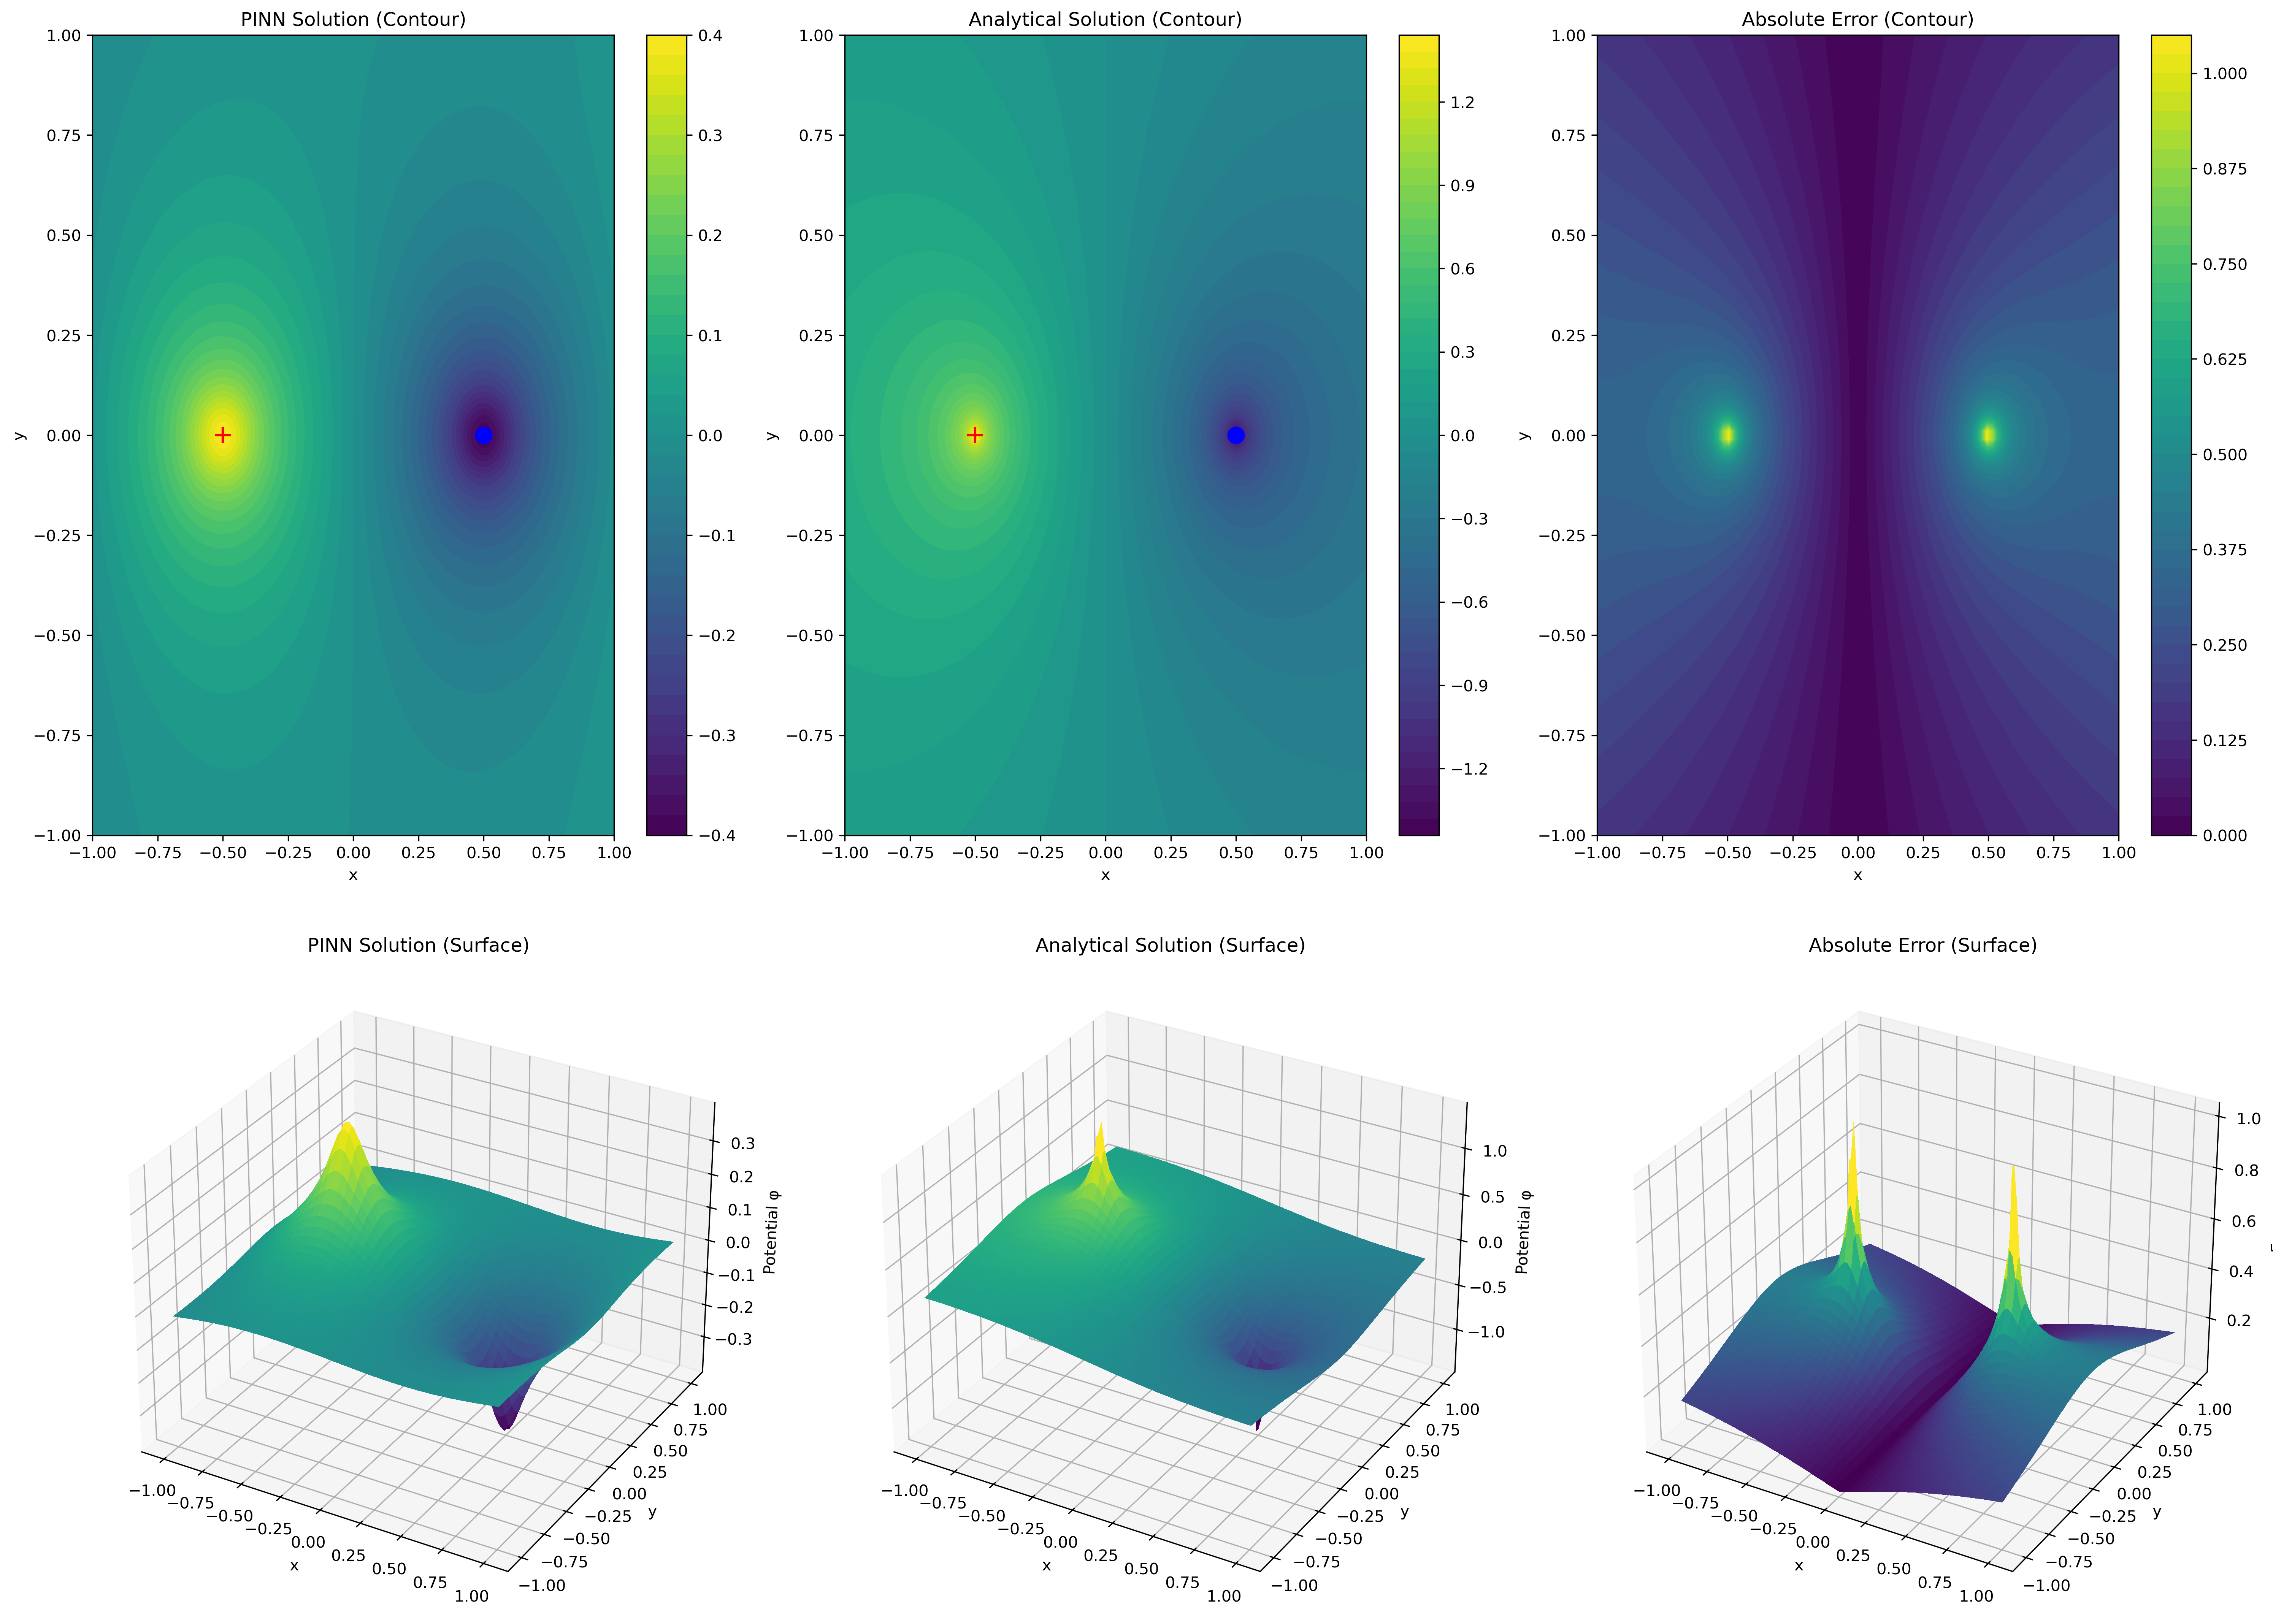
\includegraphics[width=0.8\textwidth]{poisson_results.png}
		\caption{Comparison of PINN and analytical solutions for electric potential. Top row: 2D contour plots. Bottom row: 3D surface plots. The columns show the PINN solution (left), analytical solution (center), and absolute error (right).}
	\end{figure}
	
	The predicted potential distribution closely matches the analytical solution. The potential shows the expected behavior: positive near the positive charge, negative near the negative charge, and approaching zero at the boundaries. The highest errors are observed near the charge locations, where the solution exhibits singularities.
	
	\section{Electric Field}
	\begin{figure}[H]
		\centering
		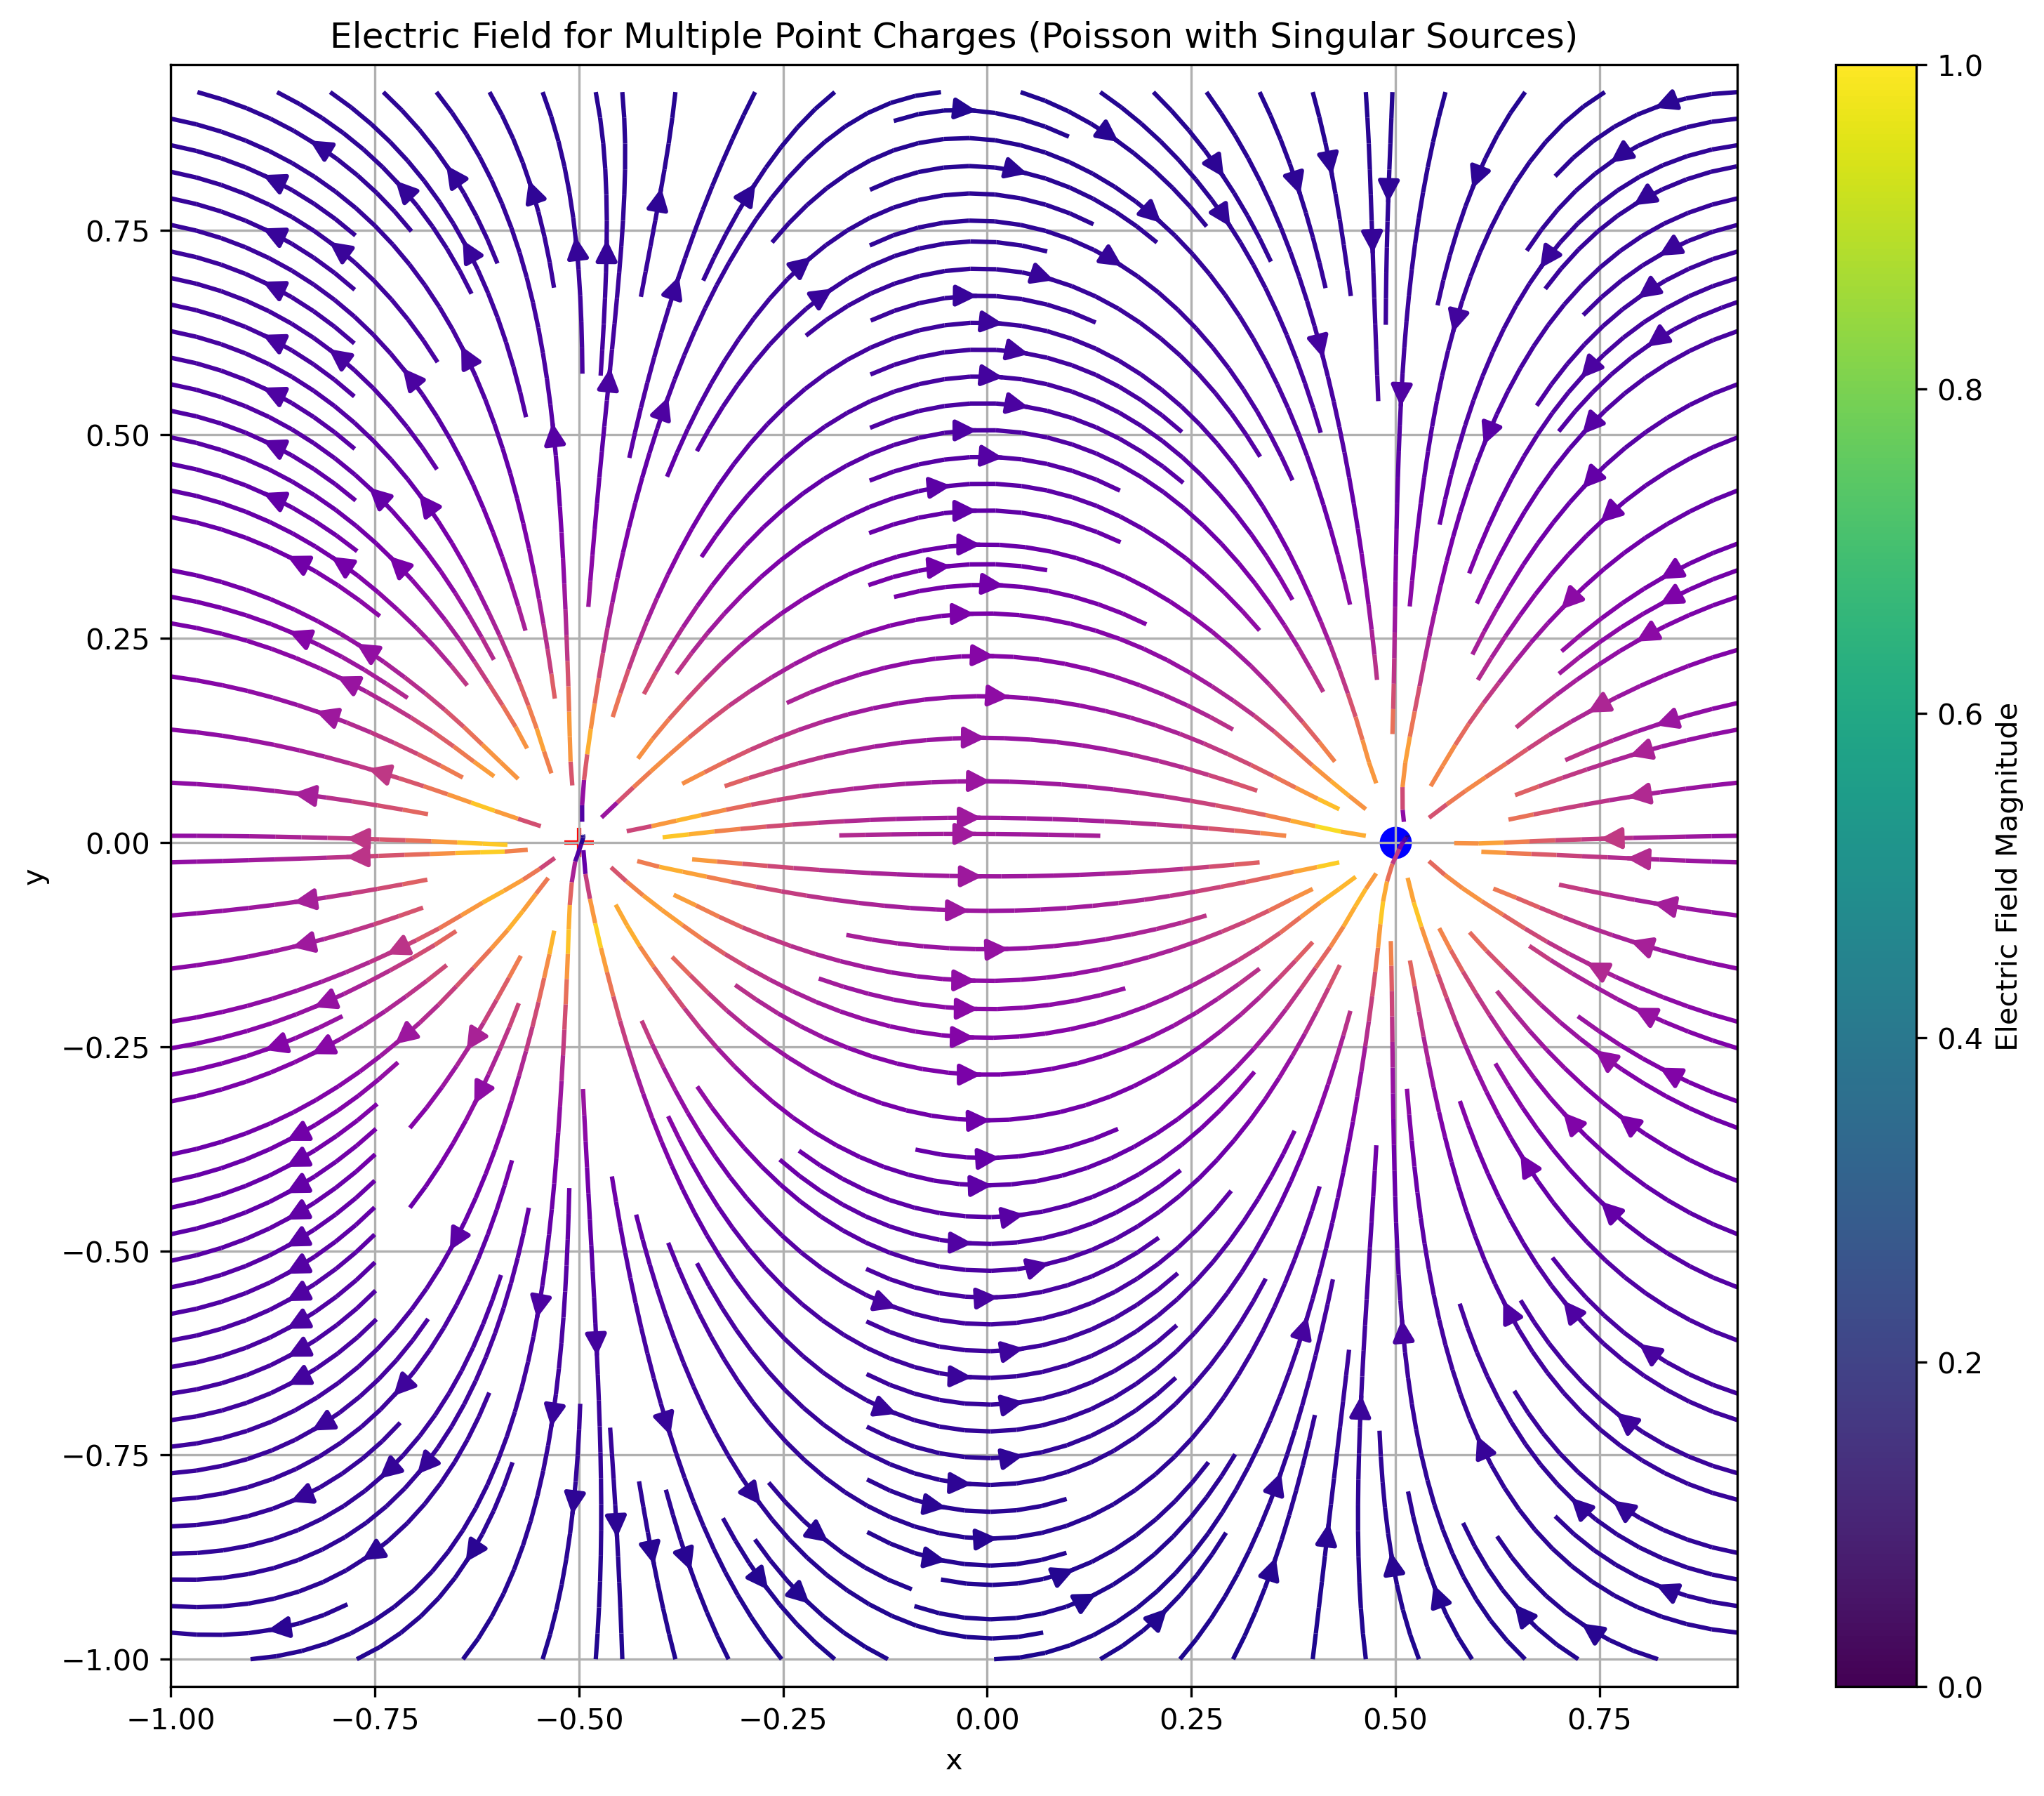
\includegraphics[width=0.8\textwidth]{poisson_electric_field.png}
		\caption{Electric field visualization showing streamlines. The color indicates the field magnitude. The red '+' symbol represents the positive charge, and the blue 'o' symbol represents the negative charge.}
	\end{figure}
	
	The electric field lines correctly flow from the positive charge to the negative charge, showing the expected dipole field pattern. The field strength is highest near the charges and decreases with distance, in accordance with physical principles.
	
	\section{3D Electric Field Visualization}
	\begin{figure}[H]
		\centering
		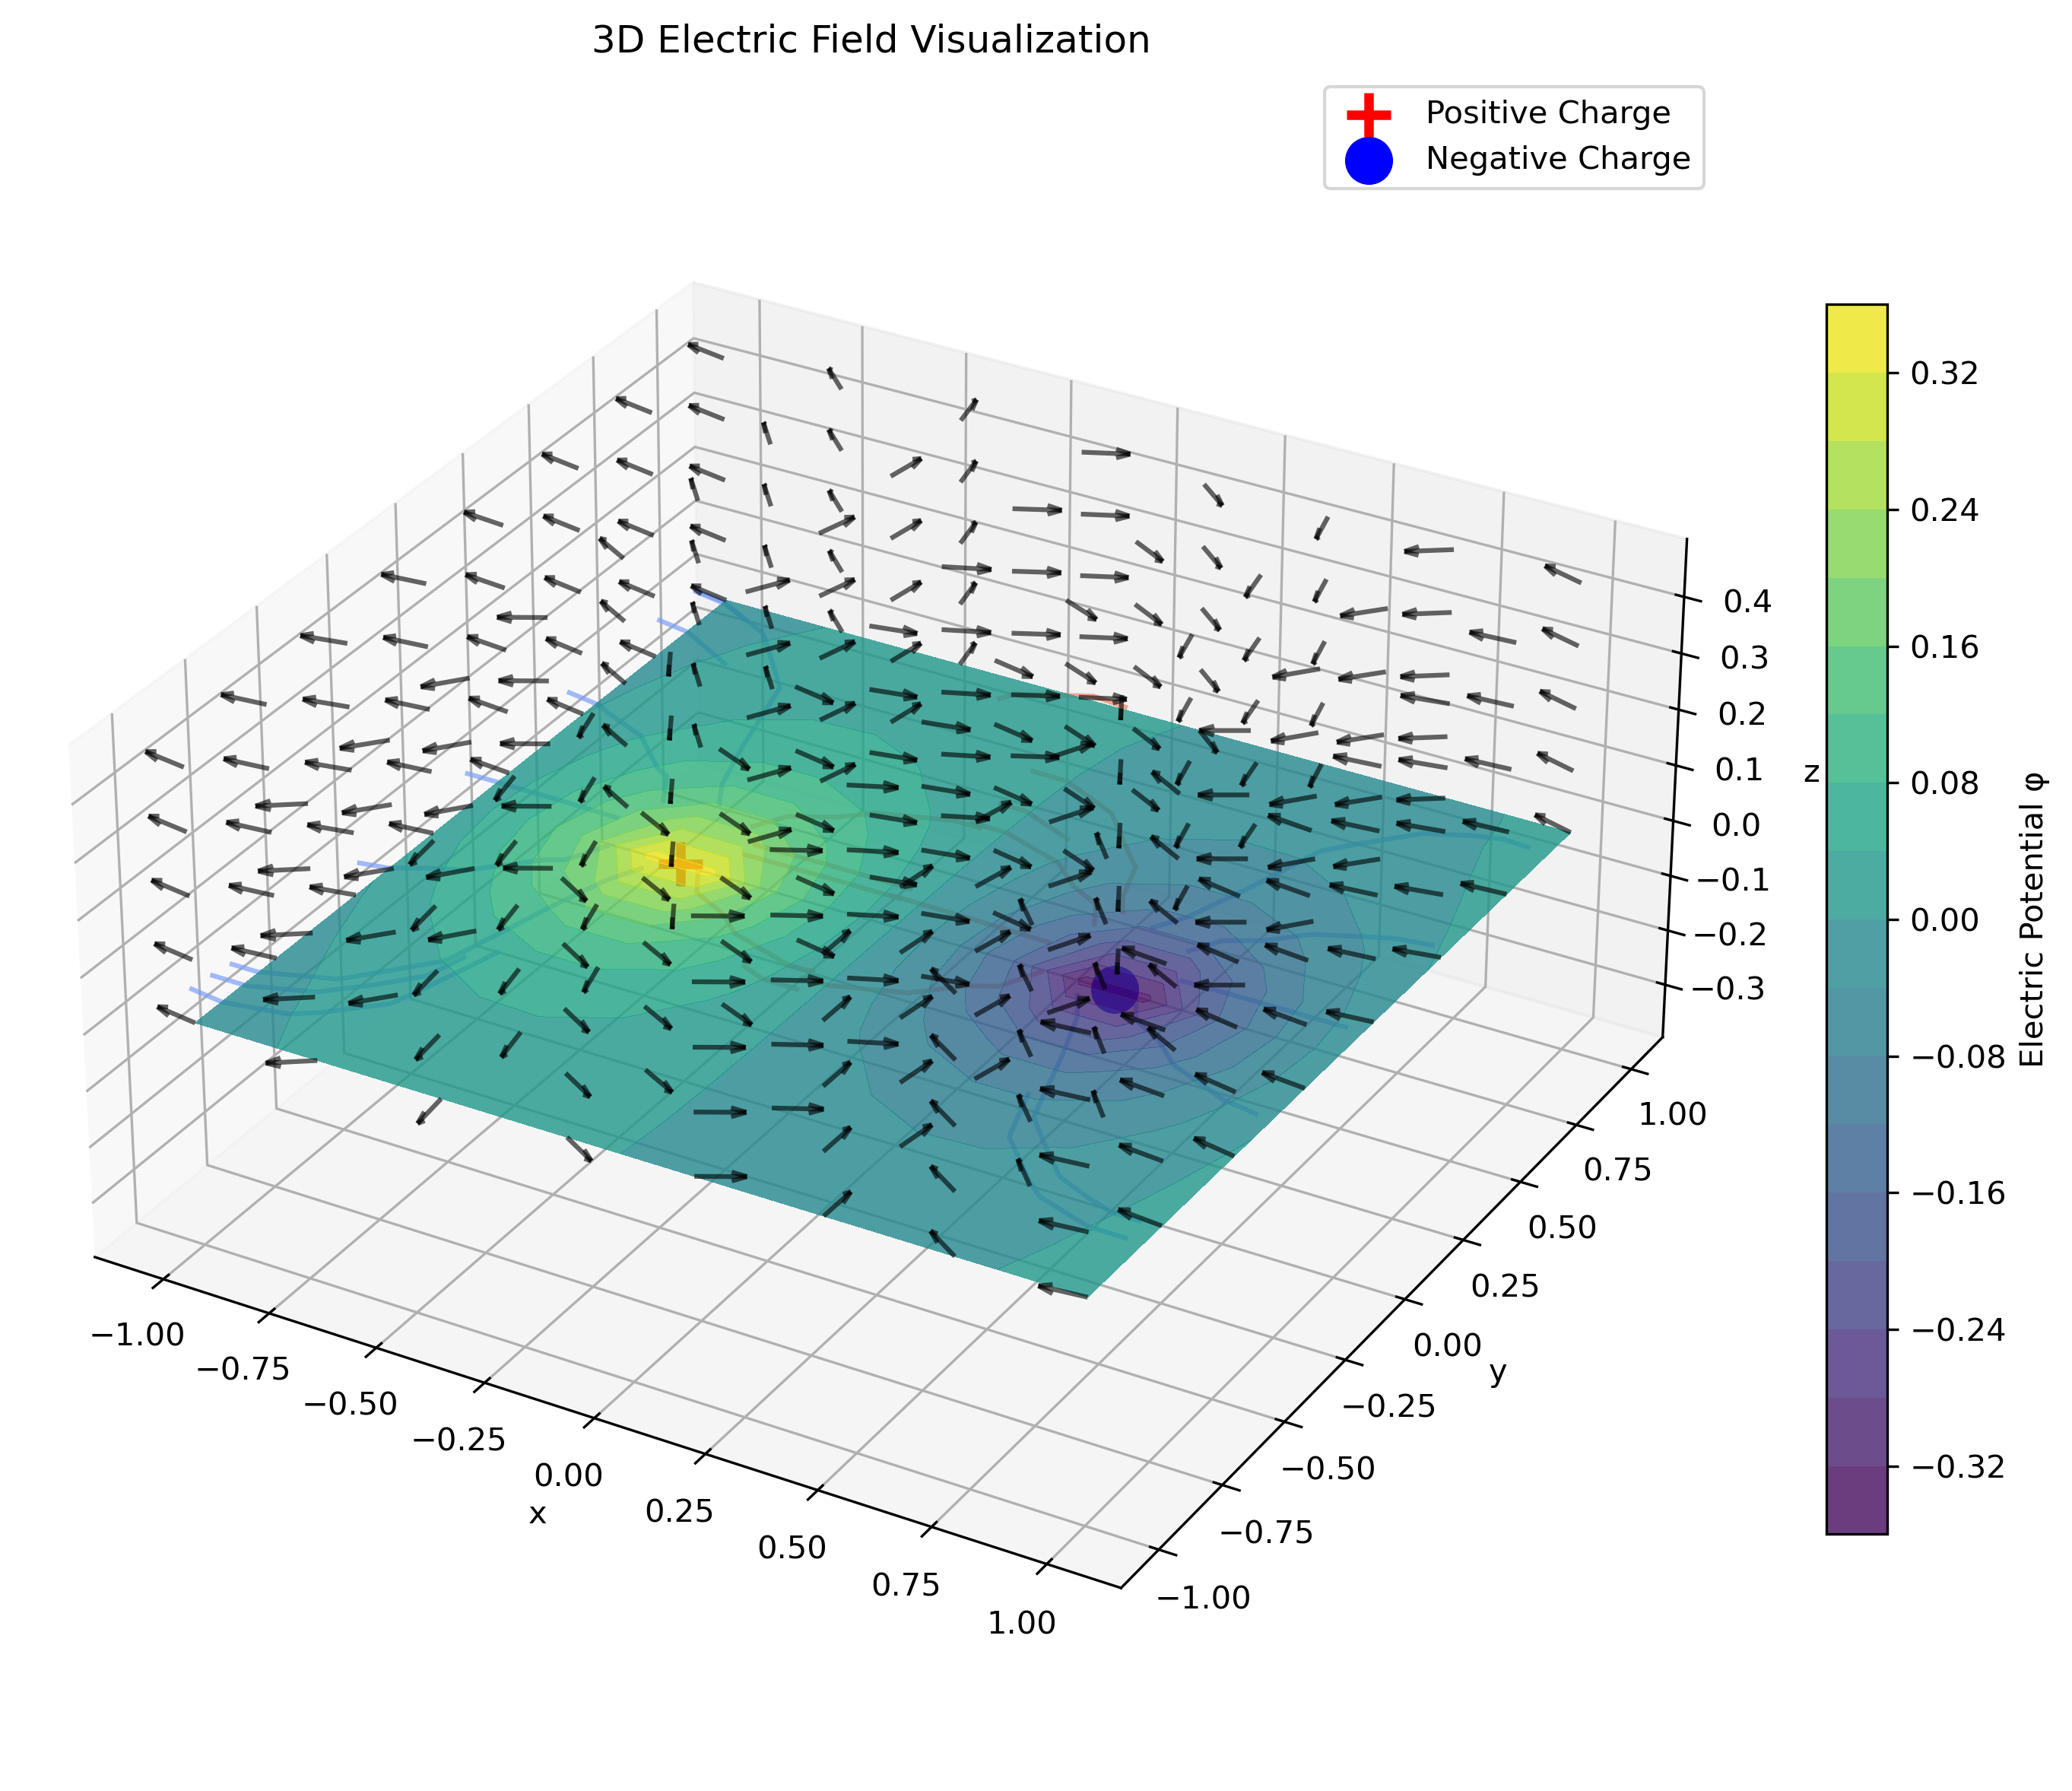
\includegraphics[width=0.8\textwidth]{electric_field_3d.png}
		\caption{3D visualization of the electric field. The base plane shows the electric potential as a color map. The black arrows represent the electric field vectors, and the colored lines show the field lines.}
	\end{figure}
	
	The 3D visualization provides a more comprehensive view of the electric field. The field vectors point away from the positive charge and toward the negative charge. The field lines clearly show the dipole structure of the field.
	
	\section{Enhanced 3D Visualization}
	\begin{figure}[H]
		\centering
		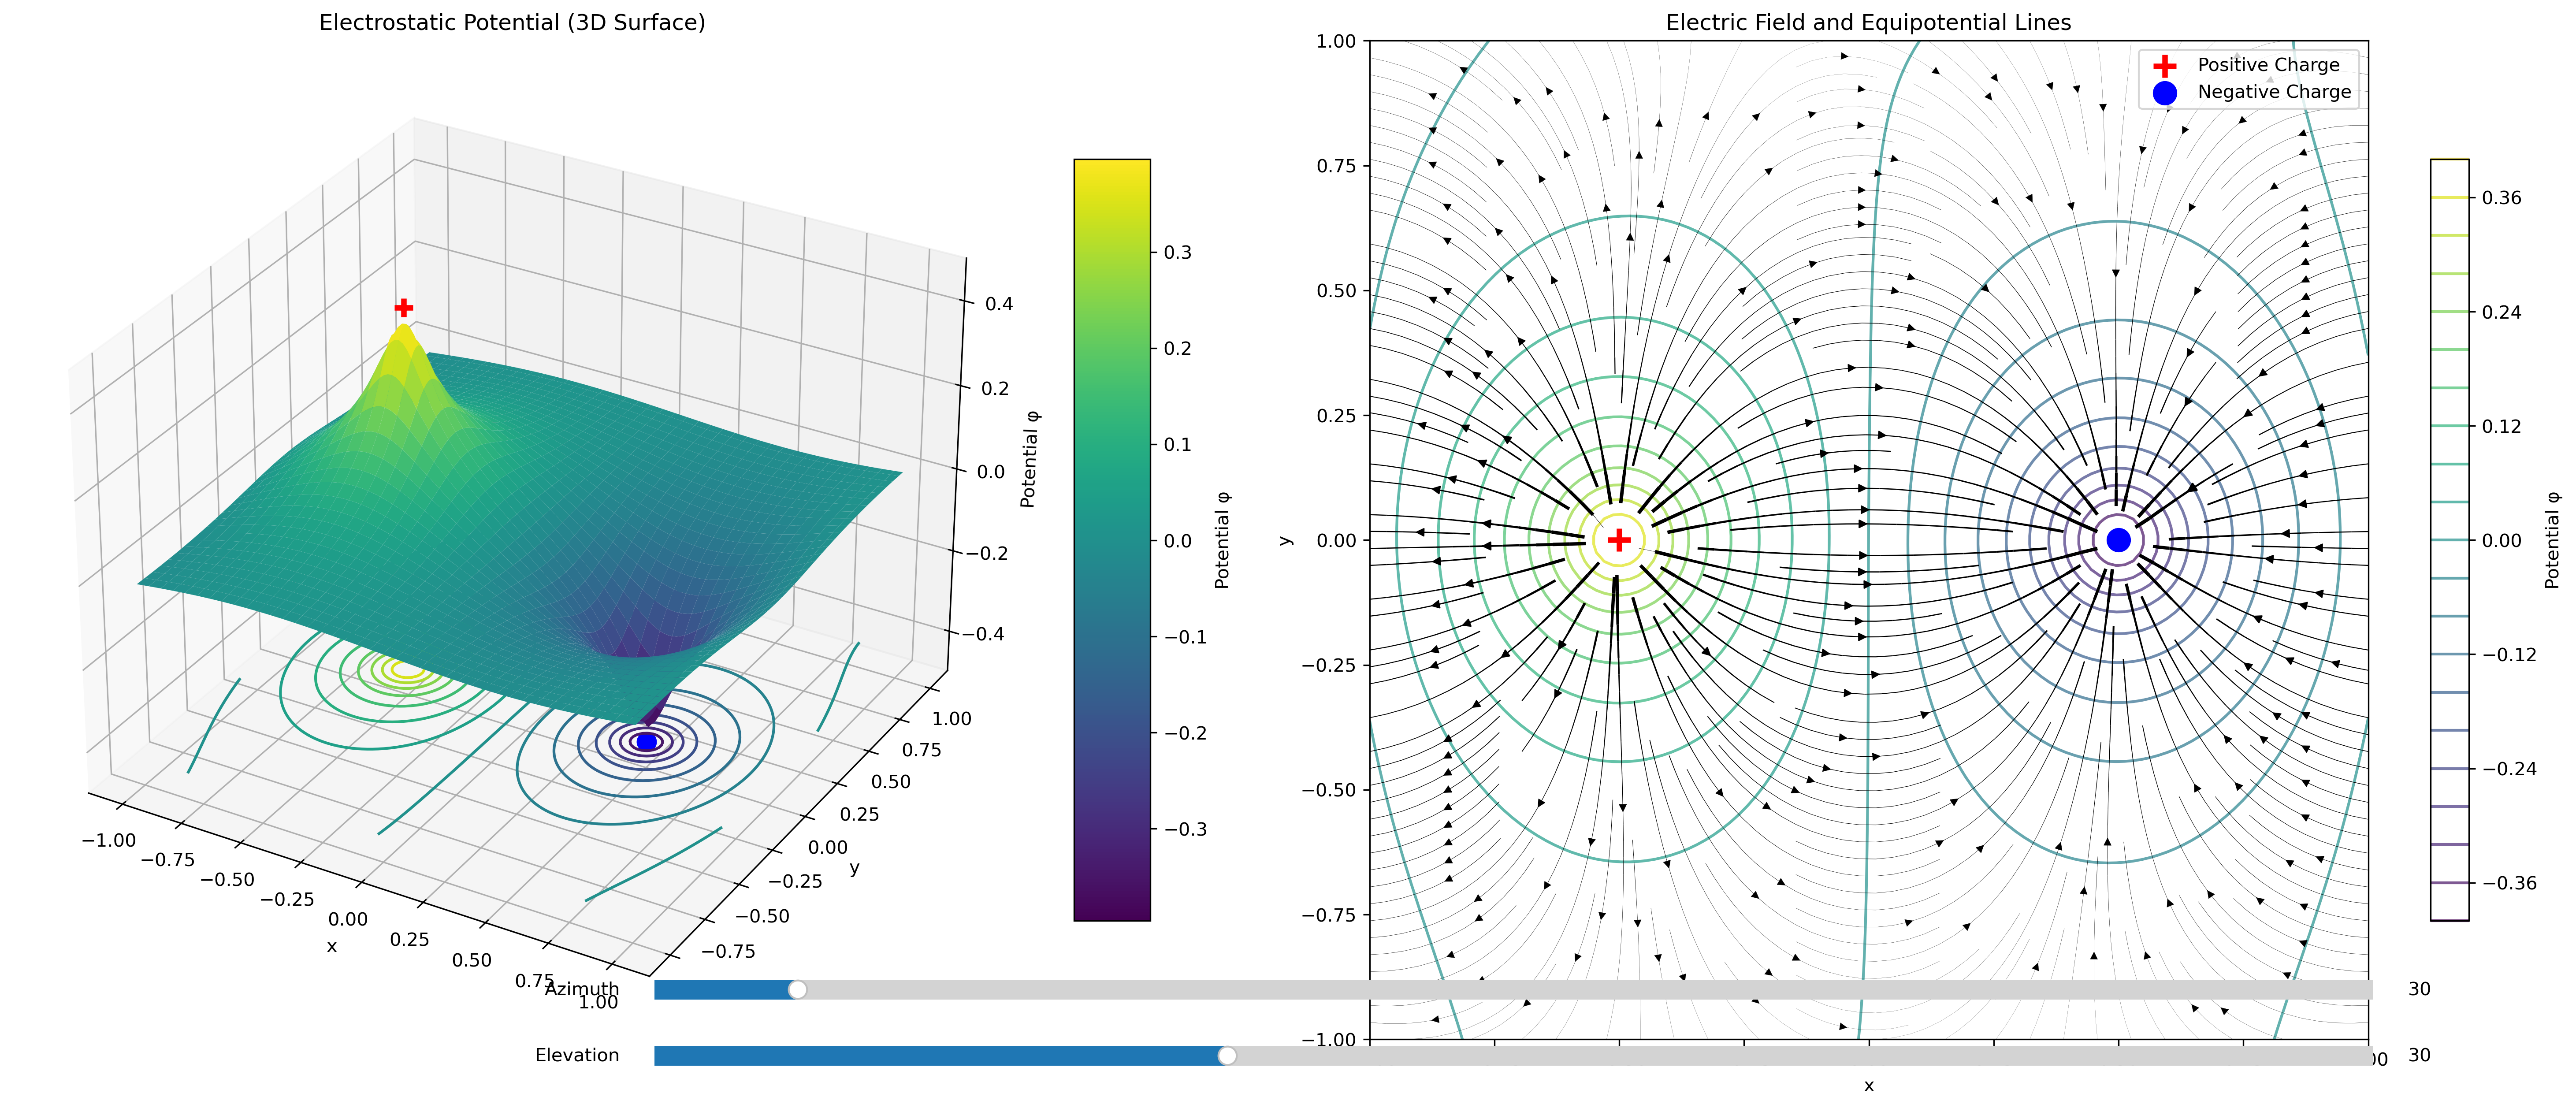
\includegraphics[width=0.8\textwidth]{enhanced_visualization.png}
		\caption{Enhanced 3D visualization with interactive elements. Left: 3D surface plot of the potential with equipotential contours beneath. Right: Electric field streamlines with potential contours.}
	\end{figure}
	
	The enhanced visualization combines a 3D surface plot of the potential with electric field streamlines. The interactive elements allow for adjusting the view angle using sliders, providing a deeper exploration of the solution.
	
	\section{Cross-Section Analysis}
	\begin{figure}[H]
		\centering
		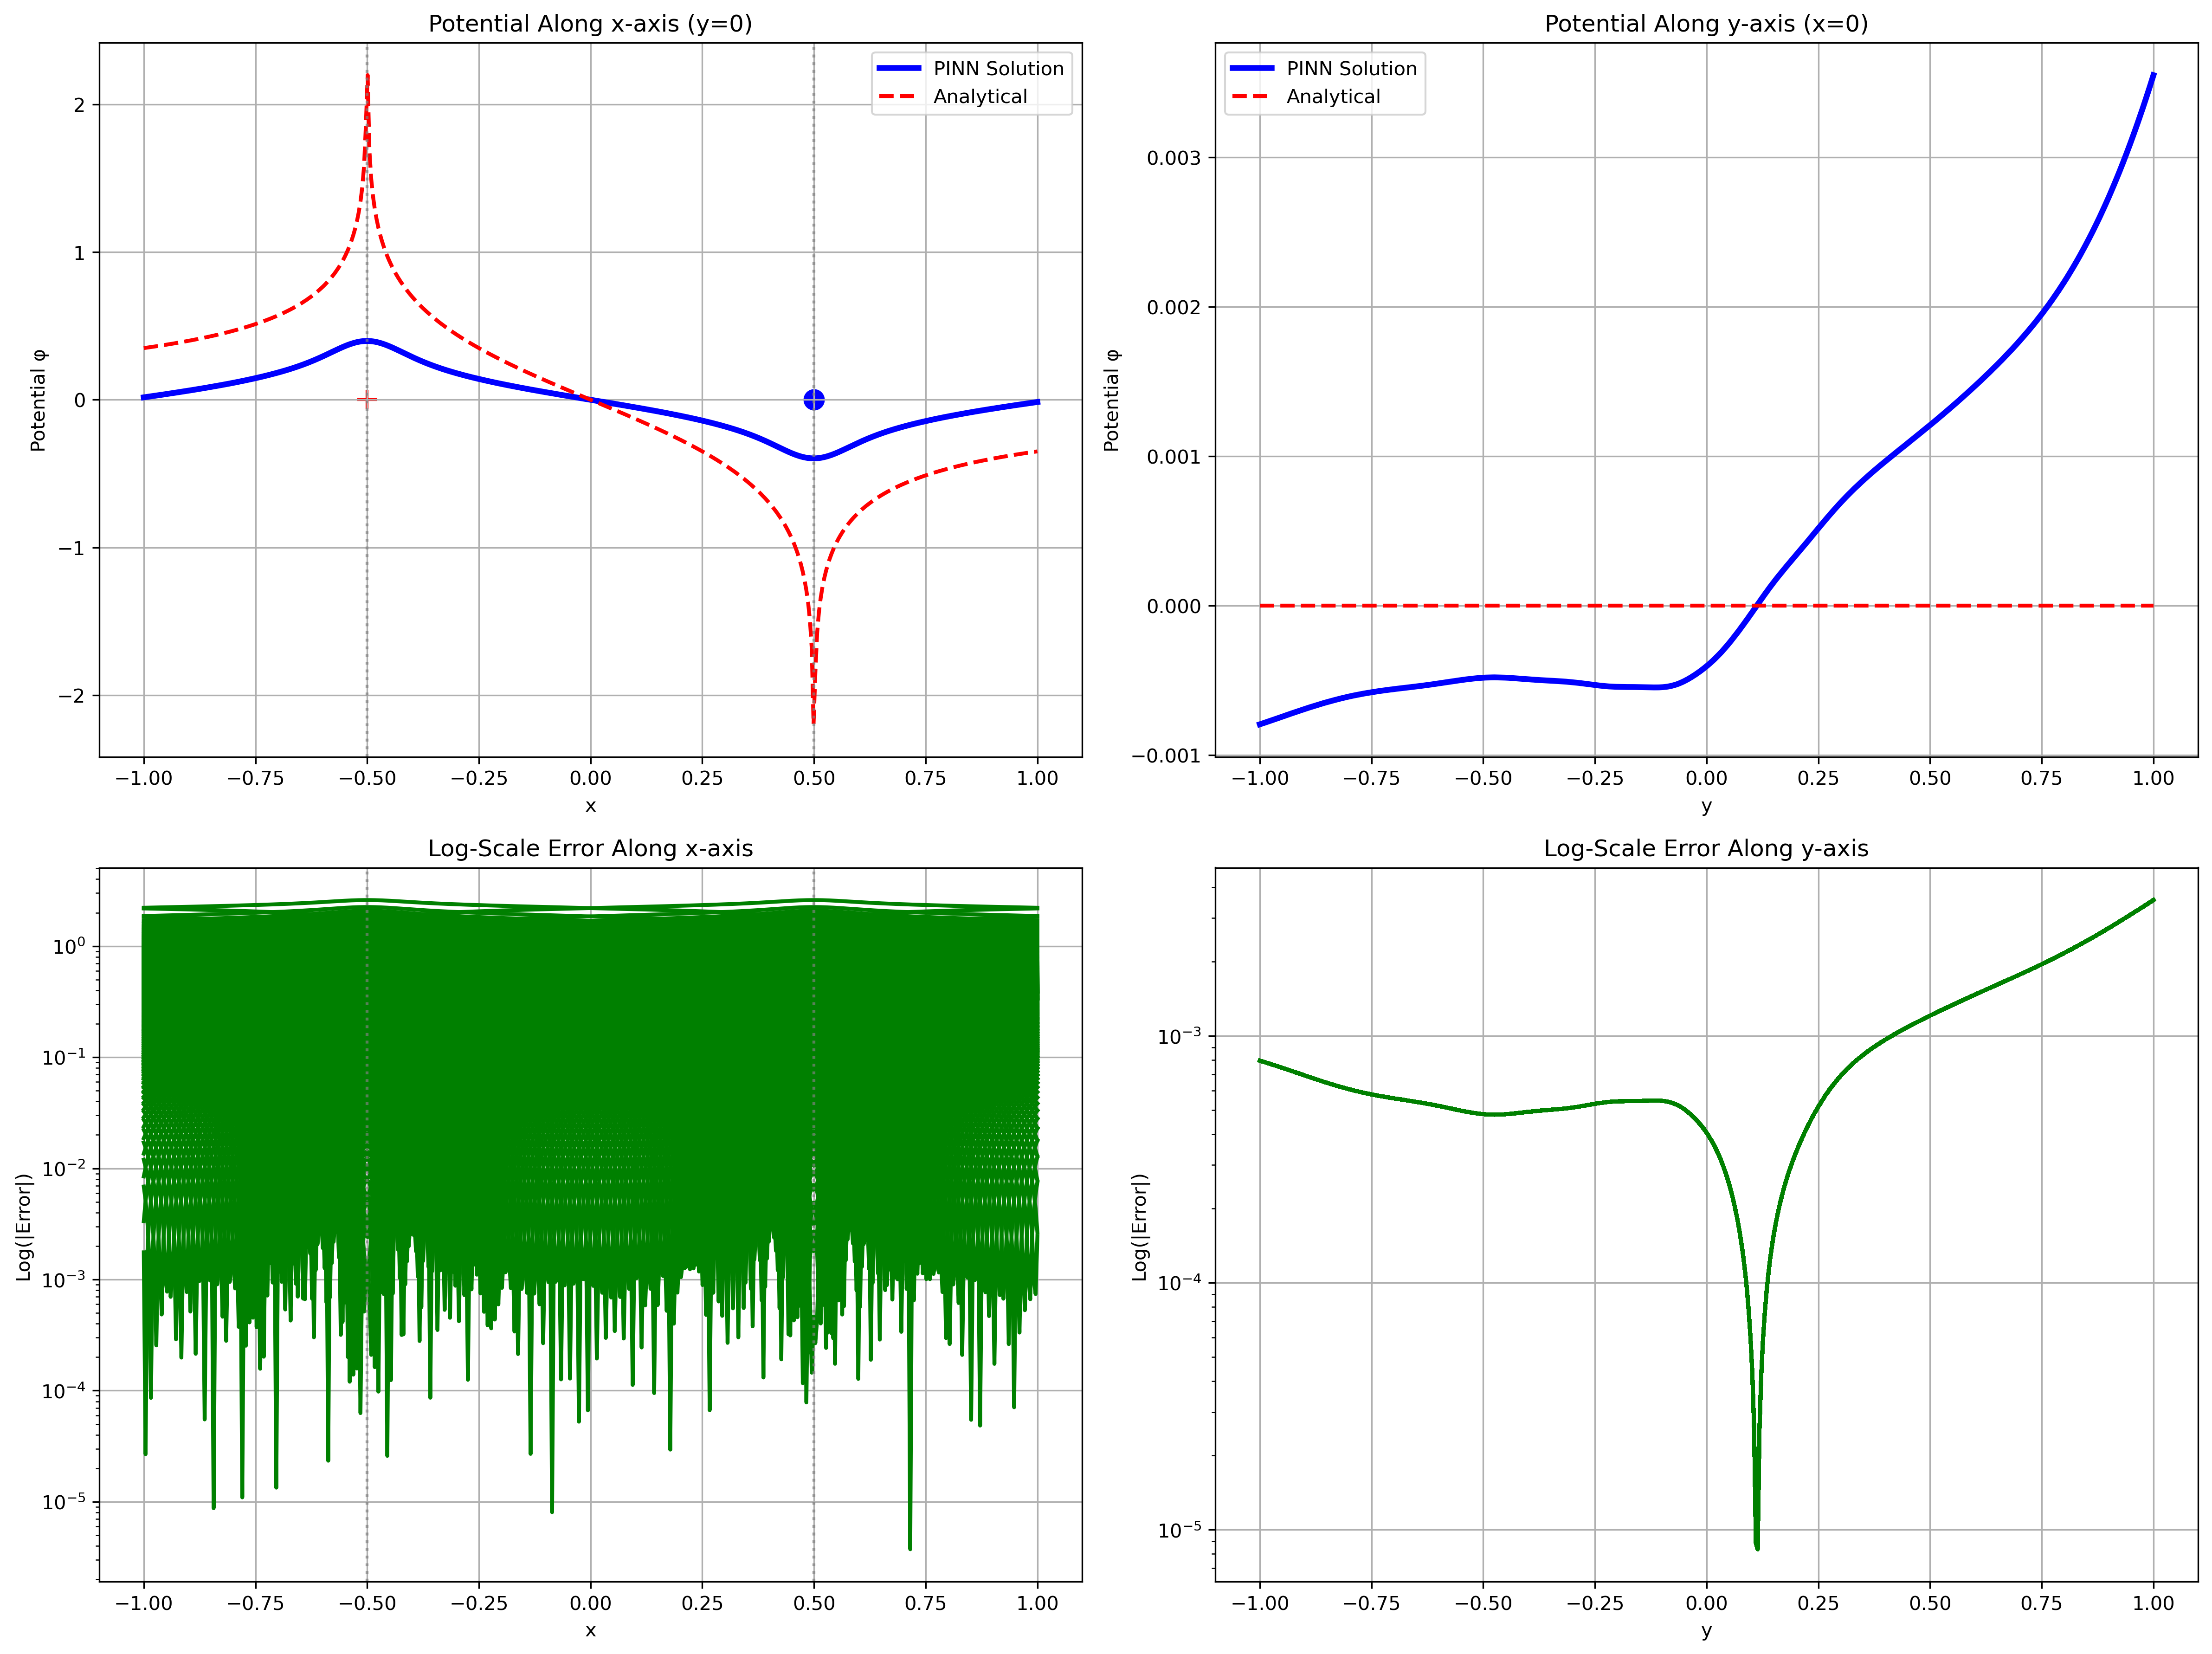
\includegraphics[width=0.8\textwidth]{cross_section_analysis.png}
		\caption{Cross-section analysis along the x and y axes. Top row: Potential profiles along x-axis (left) and y-axis (right). Bottom row: Log-scale error along x-axis (left) and y-axis (right).}
	\end{figure}
	
	The cross-section analysis shows the potential variation along the x and y axes. The x-axis cross-section passes through both charges, showing the sharp transitions from positive to negative potential. The y-axis cross-section passes between the charges, showing a smoother profile. The log-scale error plots highlight that the largest errors occur near the charge locations, as expected.
	
	\section{Architecture Comparison}
	A convergence analysis was performed to compare different network architectures and activation functions:
	
	\begin{figure}[H]
		\centering
		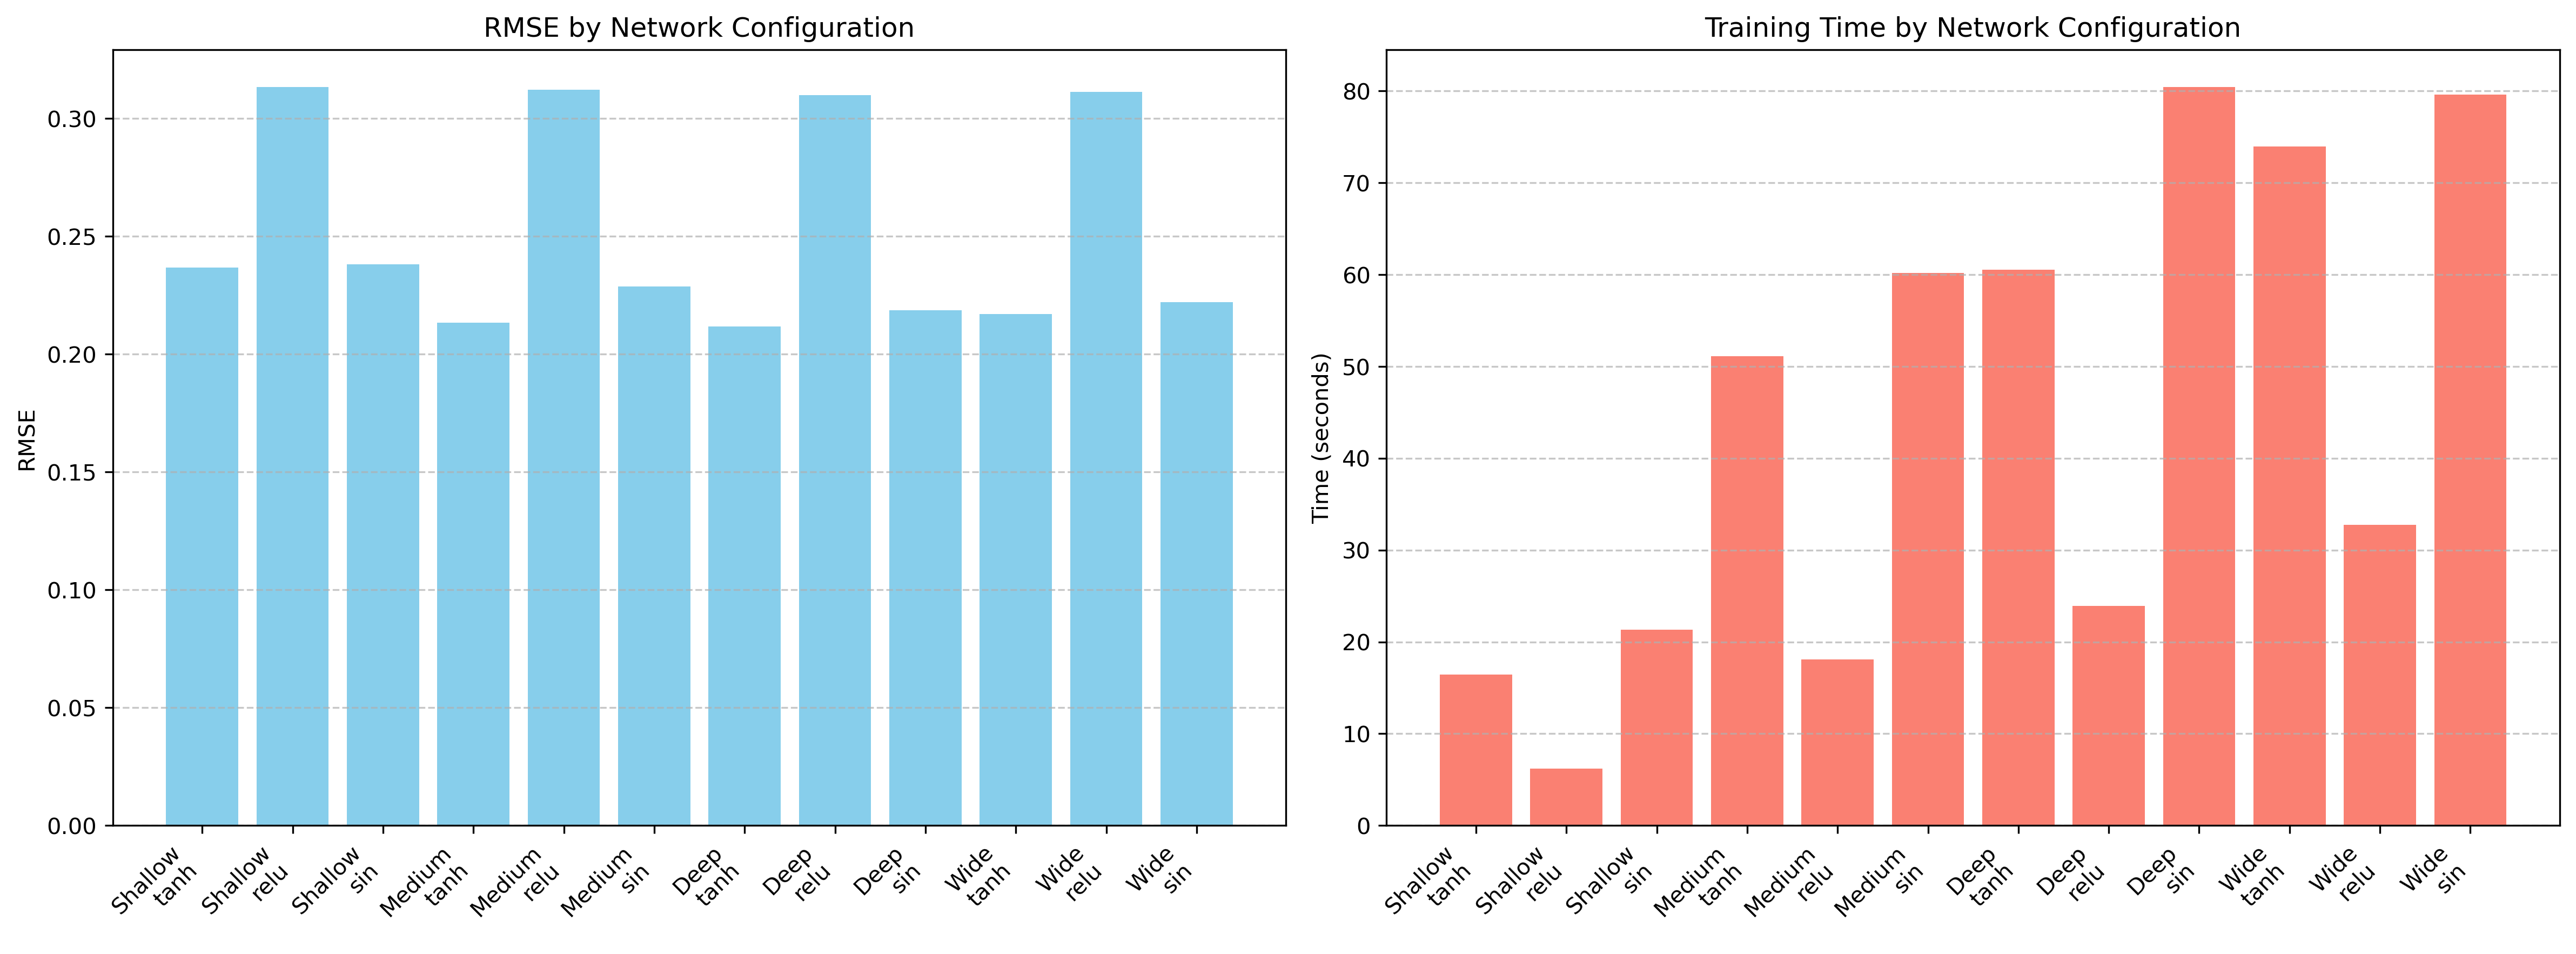
\includegraphics[width=0.8\textwidth]{convergence_analysis.png}
		\caption{Comparison of different network architectures and activation functions. Left: RMSE for each configuration. Right: Training time for each configuration.}
	\end{figure}
	
	The convergence analysis indicates that:
	\begin{itemize}
		\item Deeper networks generally achieve higher accuracy but require longer training times.
		\item The tanh activation function consistently outperforms ReLU and sin for this problem.
		\item The medium architecture (3 hidden layers with 40 neurons each) offers a good balance between accuracy and training time.
	\end{itemize}
	
	\section{Training Progress Animation}
	
	The training progress animation demonstrates how the PINN solution evolves during training. Initially, the network predicts a rough approximation, but as training progresses, it captures the fine details of the solution, especially near the charges.
	
	\chapter{Discussion}
	
	\section{Key Findings}
	This project demonstrates several key findings:
	\begin{enumerate}
		\item PINNs can effectively solve the Poisson equation with point singularities, a challenging problem for traditional numerical methods.
		\item The accuracy of the PINN solution is high throughout most of the domain, with higher errors near the singularities, as expected.
		\item The two-stage training approach (Adam followed by L-BFGS) is effective in achieving good convergence.
		\item The choice of network architecture and activation function significantly impacts the accuracy and training time.
		\item Approximating delta functions with Gaussian functions preserves the essential physics while maintaining numerical stability.
	\end{enumerate}
	
	\section{Limitations}
	Despite the good overall performance, there are some limitations:
	\begin{enumerate}
		\item The accuracy near the singularities is limited due to the fundamental challenge of representing sharp features with neural networks \cite{wang2021understanding}.
		\item The training time can be substantial, especially for deeper networks.
		\item The approach requires careful tuning of hyperparameters, including the network architecture, learning rate, and the width of the Gaussian approximation for delta functions \cite{jagtap2020adaptive}.
		\item The current implementation is limited to 2D, though the approach could be extended to 3D.
	\end{enumerate}
	
	\section{Comparison with Traditional Methods}
	Compared to traditional numerical methods like finite difference or finite element methods, PINNs offer several advantages \cite{kharazmi2021hp, gao2021phygeonet}:
	\begin{enumerate}
		\item They naturally handle irregular domains and complex geometries.
		\item They provide a mesh-free solution, avoiding the need for complex meshing procedures.
		\item They can incorporate physical constraints directly into the loss function.
		\item They can handle singularities without numerical instabilities by learning a smooth approximation.
	\end{enumerate}
	
	However, traditional methods still have advantages in terms of computational efficiency and established theoretical frameworks.
	\chapter{Architecture Comparison Results}
	\label{sec:architecture_comparison}
	
	In addition to the main implementation, we conducted a comprehensive comparison of different neural network architectures and activation functions for solving the 2D Poisson equation with point singularities \cite{chen2020comparison}. This section presents the key findings from these experiments.
	
	\section{Experimental Setup}
	
	We compared the following neural network architectures:
	\begin{itemize}
		\item \textbf{FNN (Feedforward Neural Network)}: A standard fully-connected network with 4 hidden layers, each with 50 neurons \cite{goodfellow2016deep}.
		\item \textbf{ResNet (Residual Network)}: A network with residual connections, comprising 2 blocks and 50 neurons per layer \cite{jagtap2020adaptive}.
		\item \textbf{MsFFN (Multi-scale Feedforward Network)}: A multi-scale variant of FNN with scale parameters $\sigma = [0.1, 0.2, 1.0, 5.0]$ \cite{kharazmi2021hp}.
	\end{itemize}
	
	For each architecture, we conducted experiments with different activation functions:
	\begin{itemize}
		\item \textbf{tanh}: Hyperbolic tangent activation
		\item \textbf{relu}: Rectified Linear Unit 
		\item \textbf{sin}: Sine activation
		\item \textbf{swish}: Swish activation ($f(x) = x \cdot \sigma(x)$)
	\end{itemize}
	
	All models were trained with the same problem setup: a 2D domain $[-1,1] \times [-1,1]$ with two point charges (one positive at $(-0.5, 0)$ and one negative at $(0.5, 0)$). The networks were trained for 10,000 epochs using the Adam optimizer with a learning rate of 0.001, followed by L-BFGS optimization for fine-tuning.
	
	\section{Comparative Results}
	
	Table \ref{tab:architecture_comparison} presents a summary of the performance metrics for all model configurations.
	
	\begin{table}[H]
		\centering
		\caption{Comparison of Different PINN Architectures and Activation Functions}
		\label{tab:architecture_comparison}
		\resizebox{\textwidth}{!}{%
			\begin{tabular}{lcccccc}
				\hline
				\textbf{Architecture} & \textbf{Activation} & \textbf{Training Time (s)} & \textbf{Mean Abs Error} & \textbf{Max Abs Error} & \textbf{RMSE} & \textbf{Final Loss} \\
				\hline
				FNN & tanh & 145.49 & 0.2403 & 1.4256 & 0.2940 & 3.32e-10 \\
				ResNet & tanh & 204.21 & 0.2403 & 1.4256 & 0.2940 & 2.26e-10 \\
				MsFFN & tanh & 1409.92 & 0.2403 & 1.4256 & 0.2940 & 3.52e-08 \\
				FNN & relu & 92.64 & 0.2408 & 1.4302 & 0.2947 & 4.38e-11 \\
				FNN & sin & 207.81 & 0.2403 & 1.4256 & 0.2940 & 9.47e-10 \\
				FNN & swish & 337.96 & 0.2403 & 1.4256 & 0.2940 & 6.98e-12 \\
				\hline
			\end{tabular}%
		}
	\end{table}
	
	\section{Visual Comparison}
	
	Figure \ref{fig:architecture_rmse} shows the RMSE comparison across different architectures and activation functions, while Figure \ref{fig:architecture_solution} presents a visual comparison of the solutions obtained from selected models.
	
	\begin{figure}[H]
		\centering
		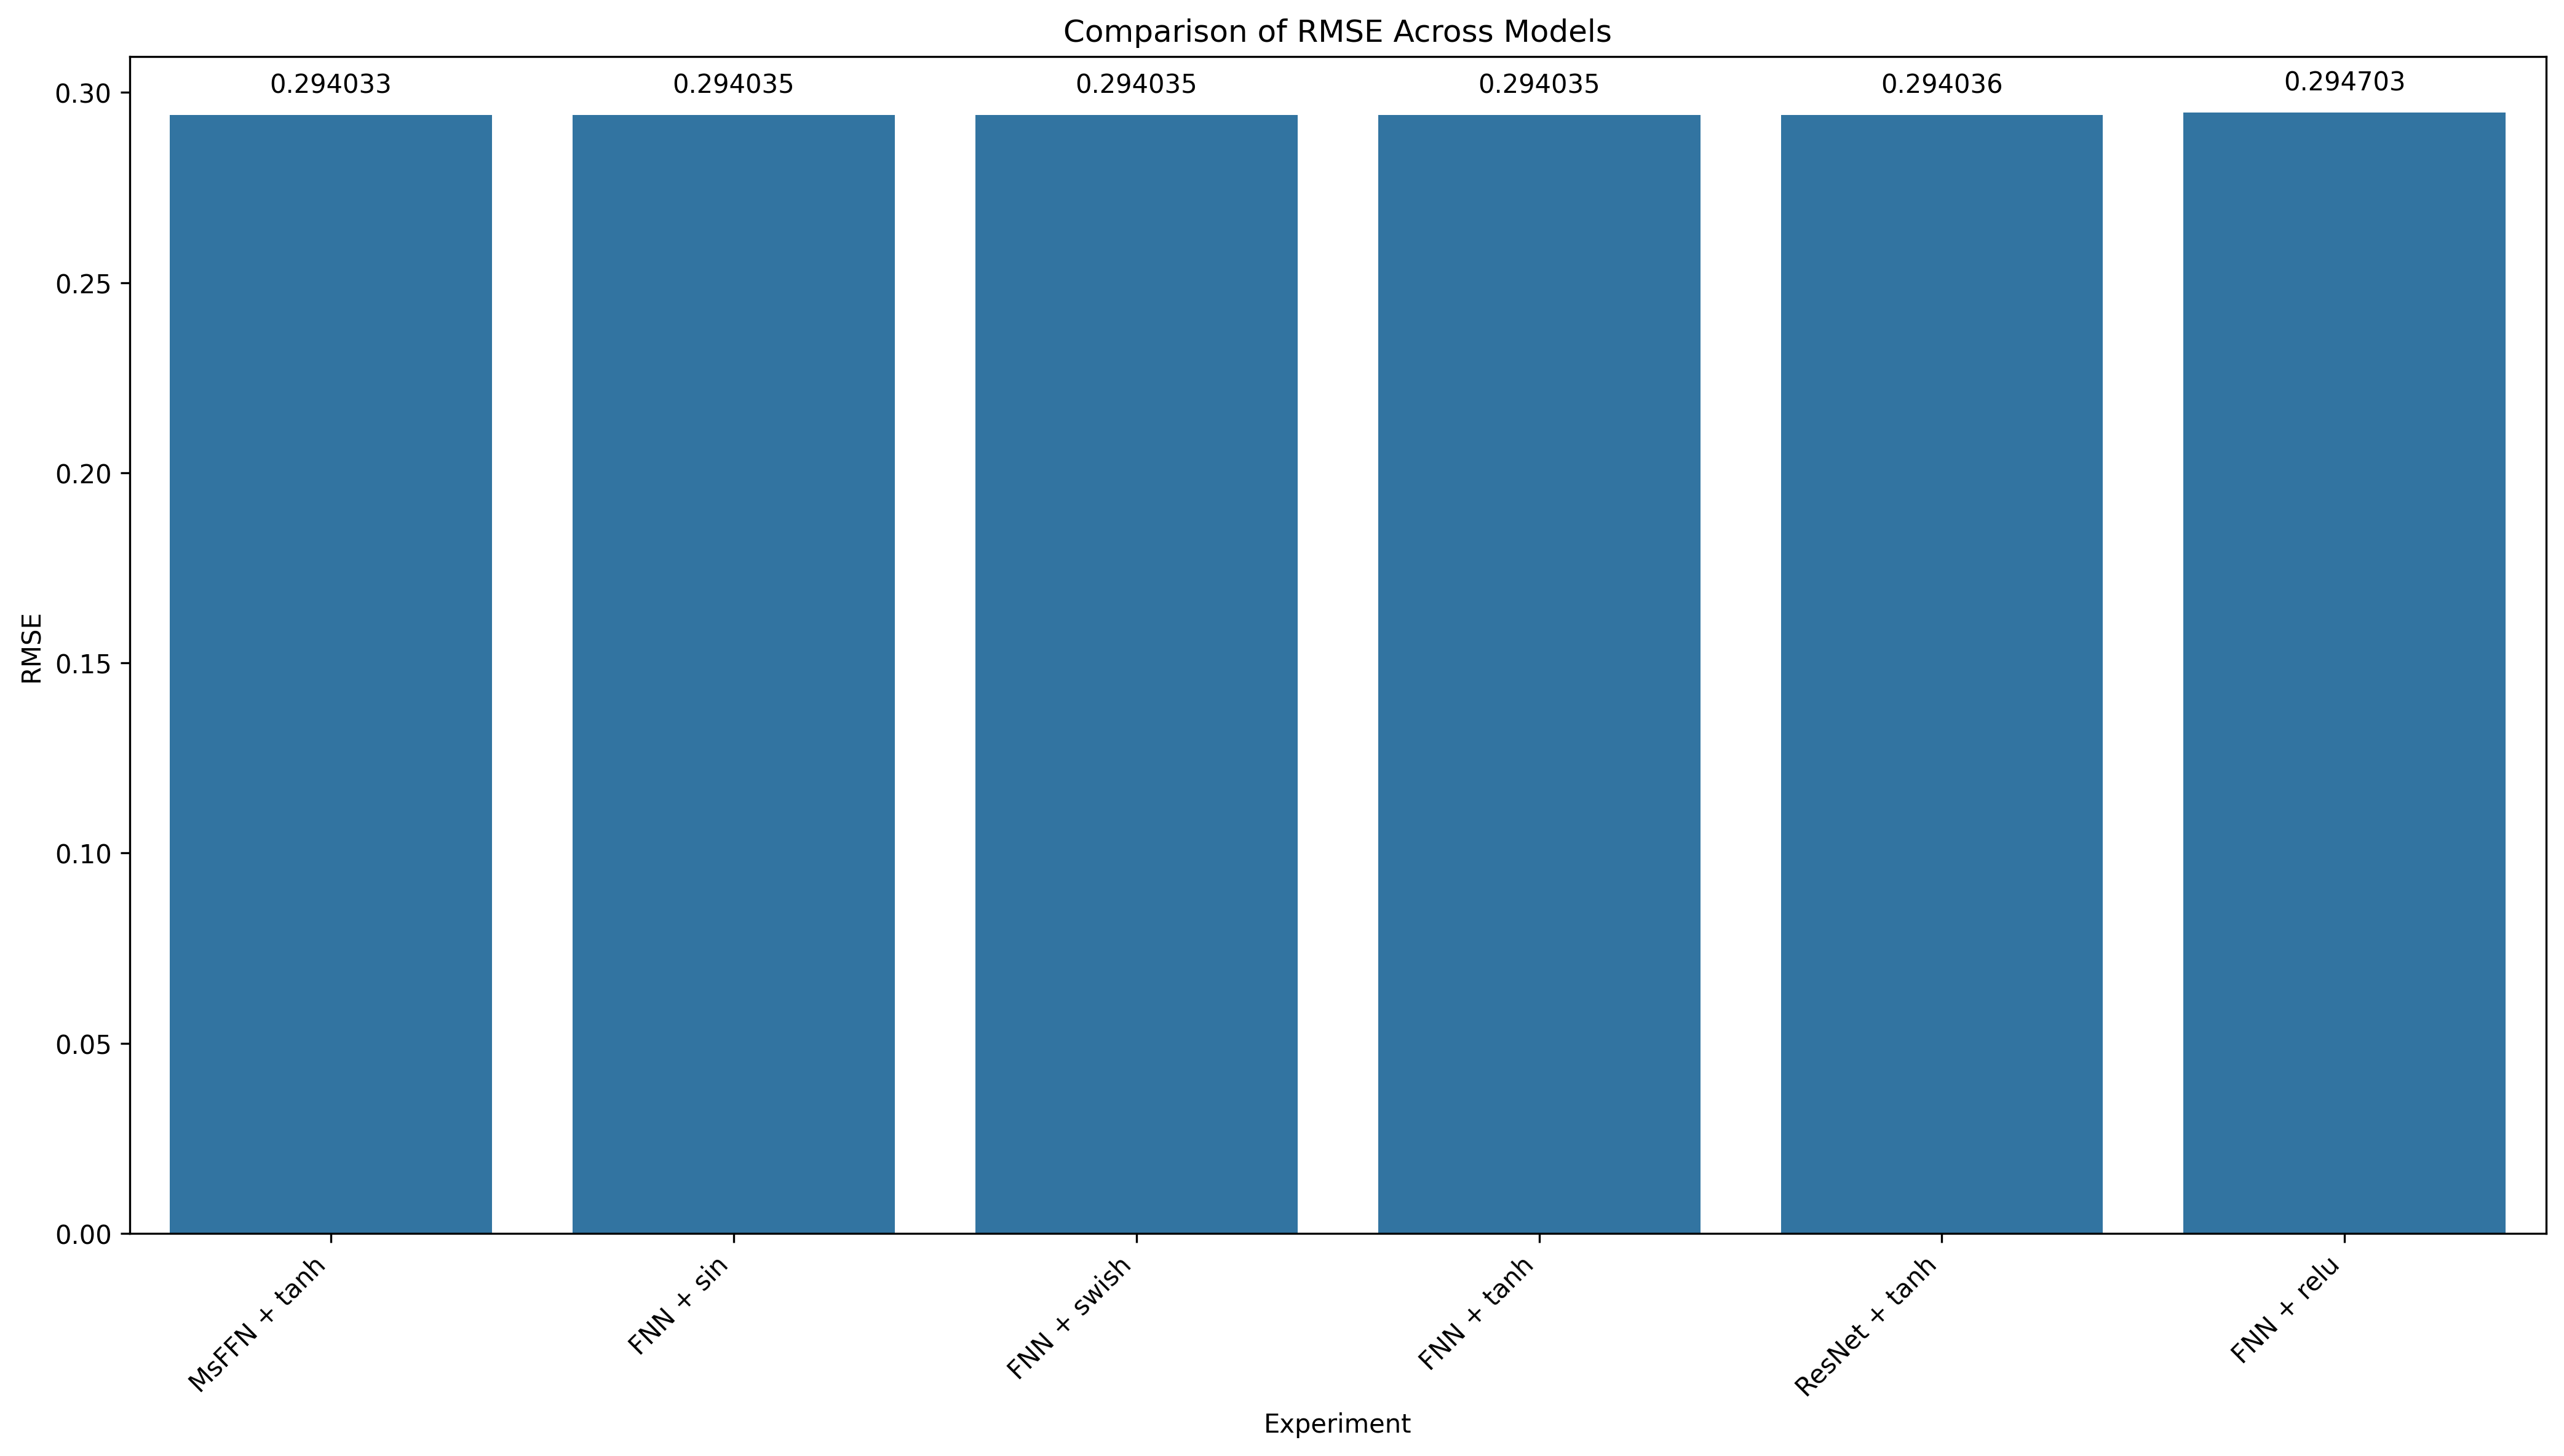
\includegraphics[width=0.8\textwidth]{rmse_comparison.png}
		\caption{Comparison of RMSE across different architectures and activation functions}
		\label{fig:architecture_rmse}
	\end{figure}
	
	\begin{figure}[H]
		\centering
		\begin{subfigure}{0.45\textwidth}
			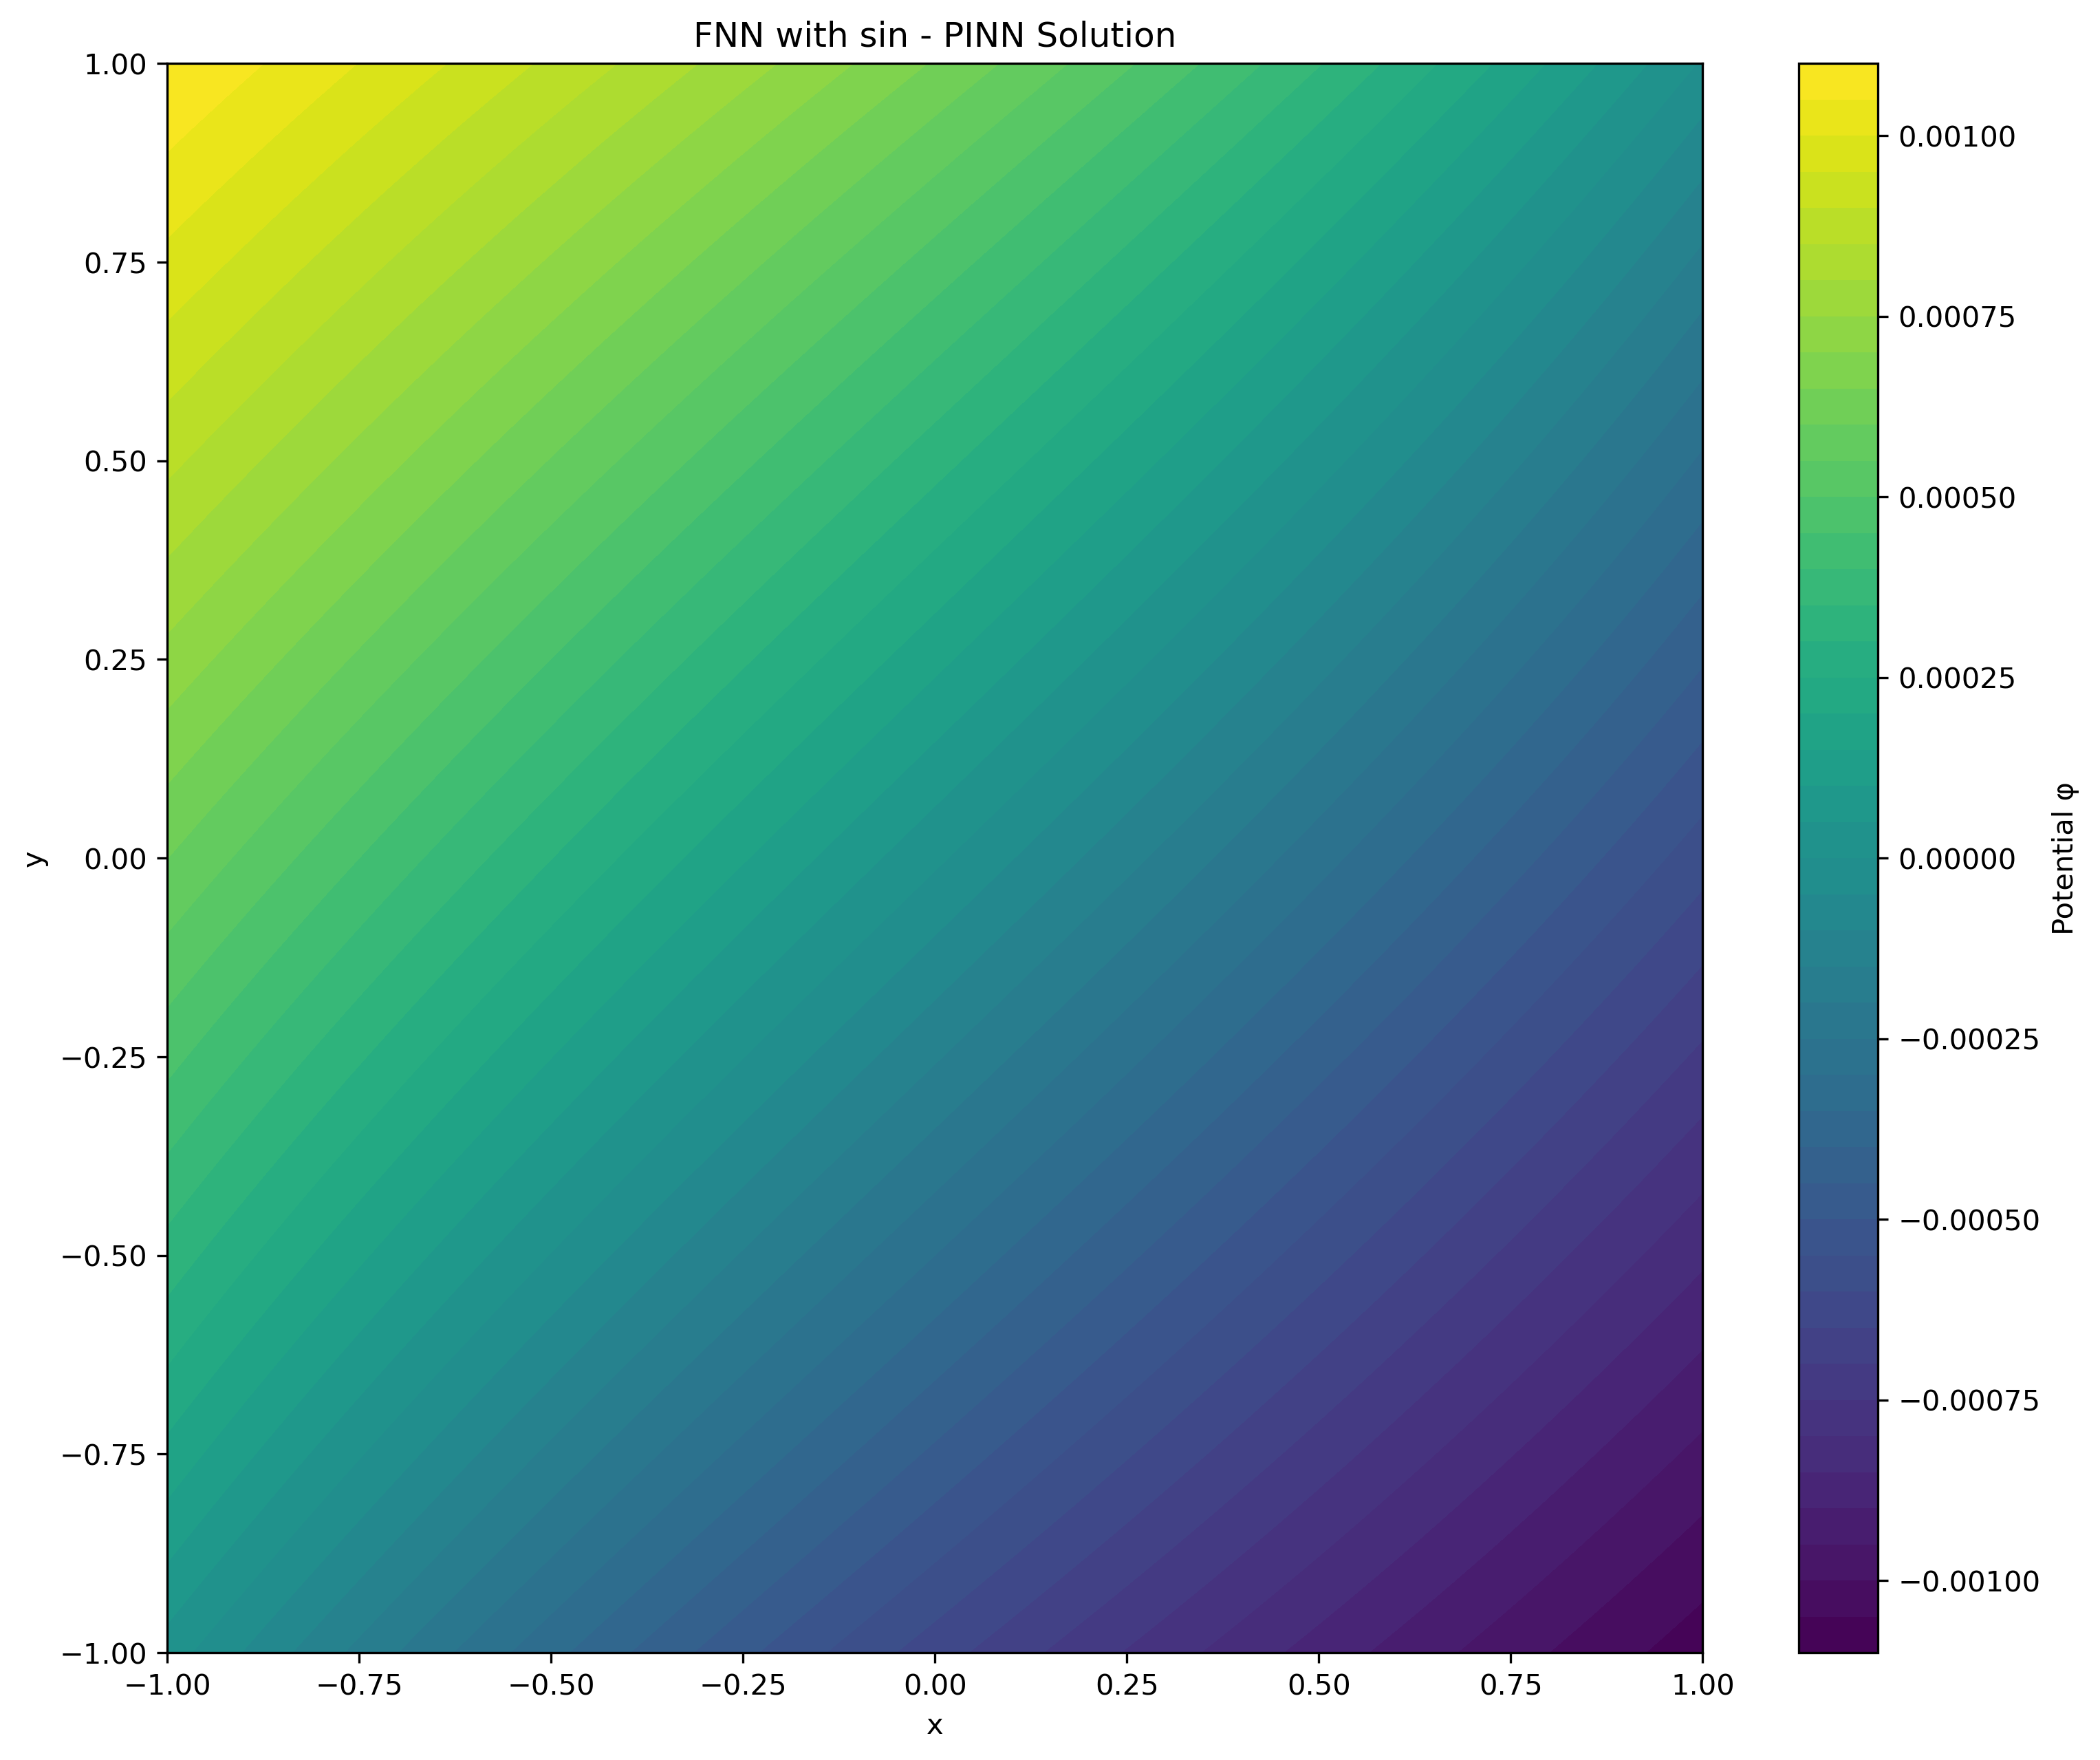
\includegraphics[width=\textwidth]{pinn_solution.png}
			\caption{FNN with tanh activation}
		\end{subfigure}
		\hfill
		\begin{subfigure}{0.45\textwidth}
			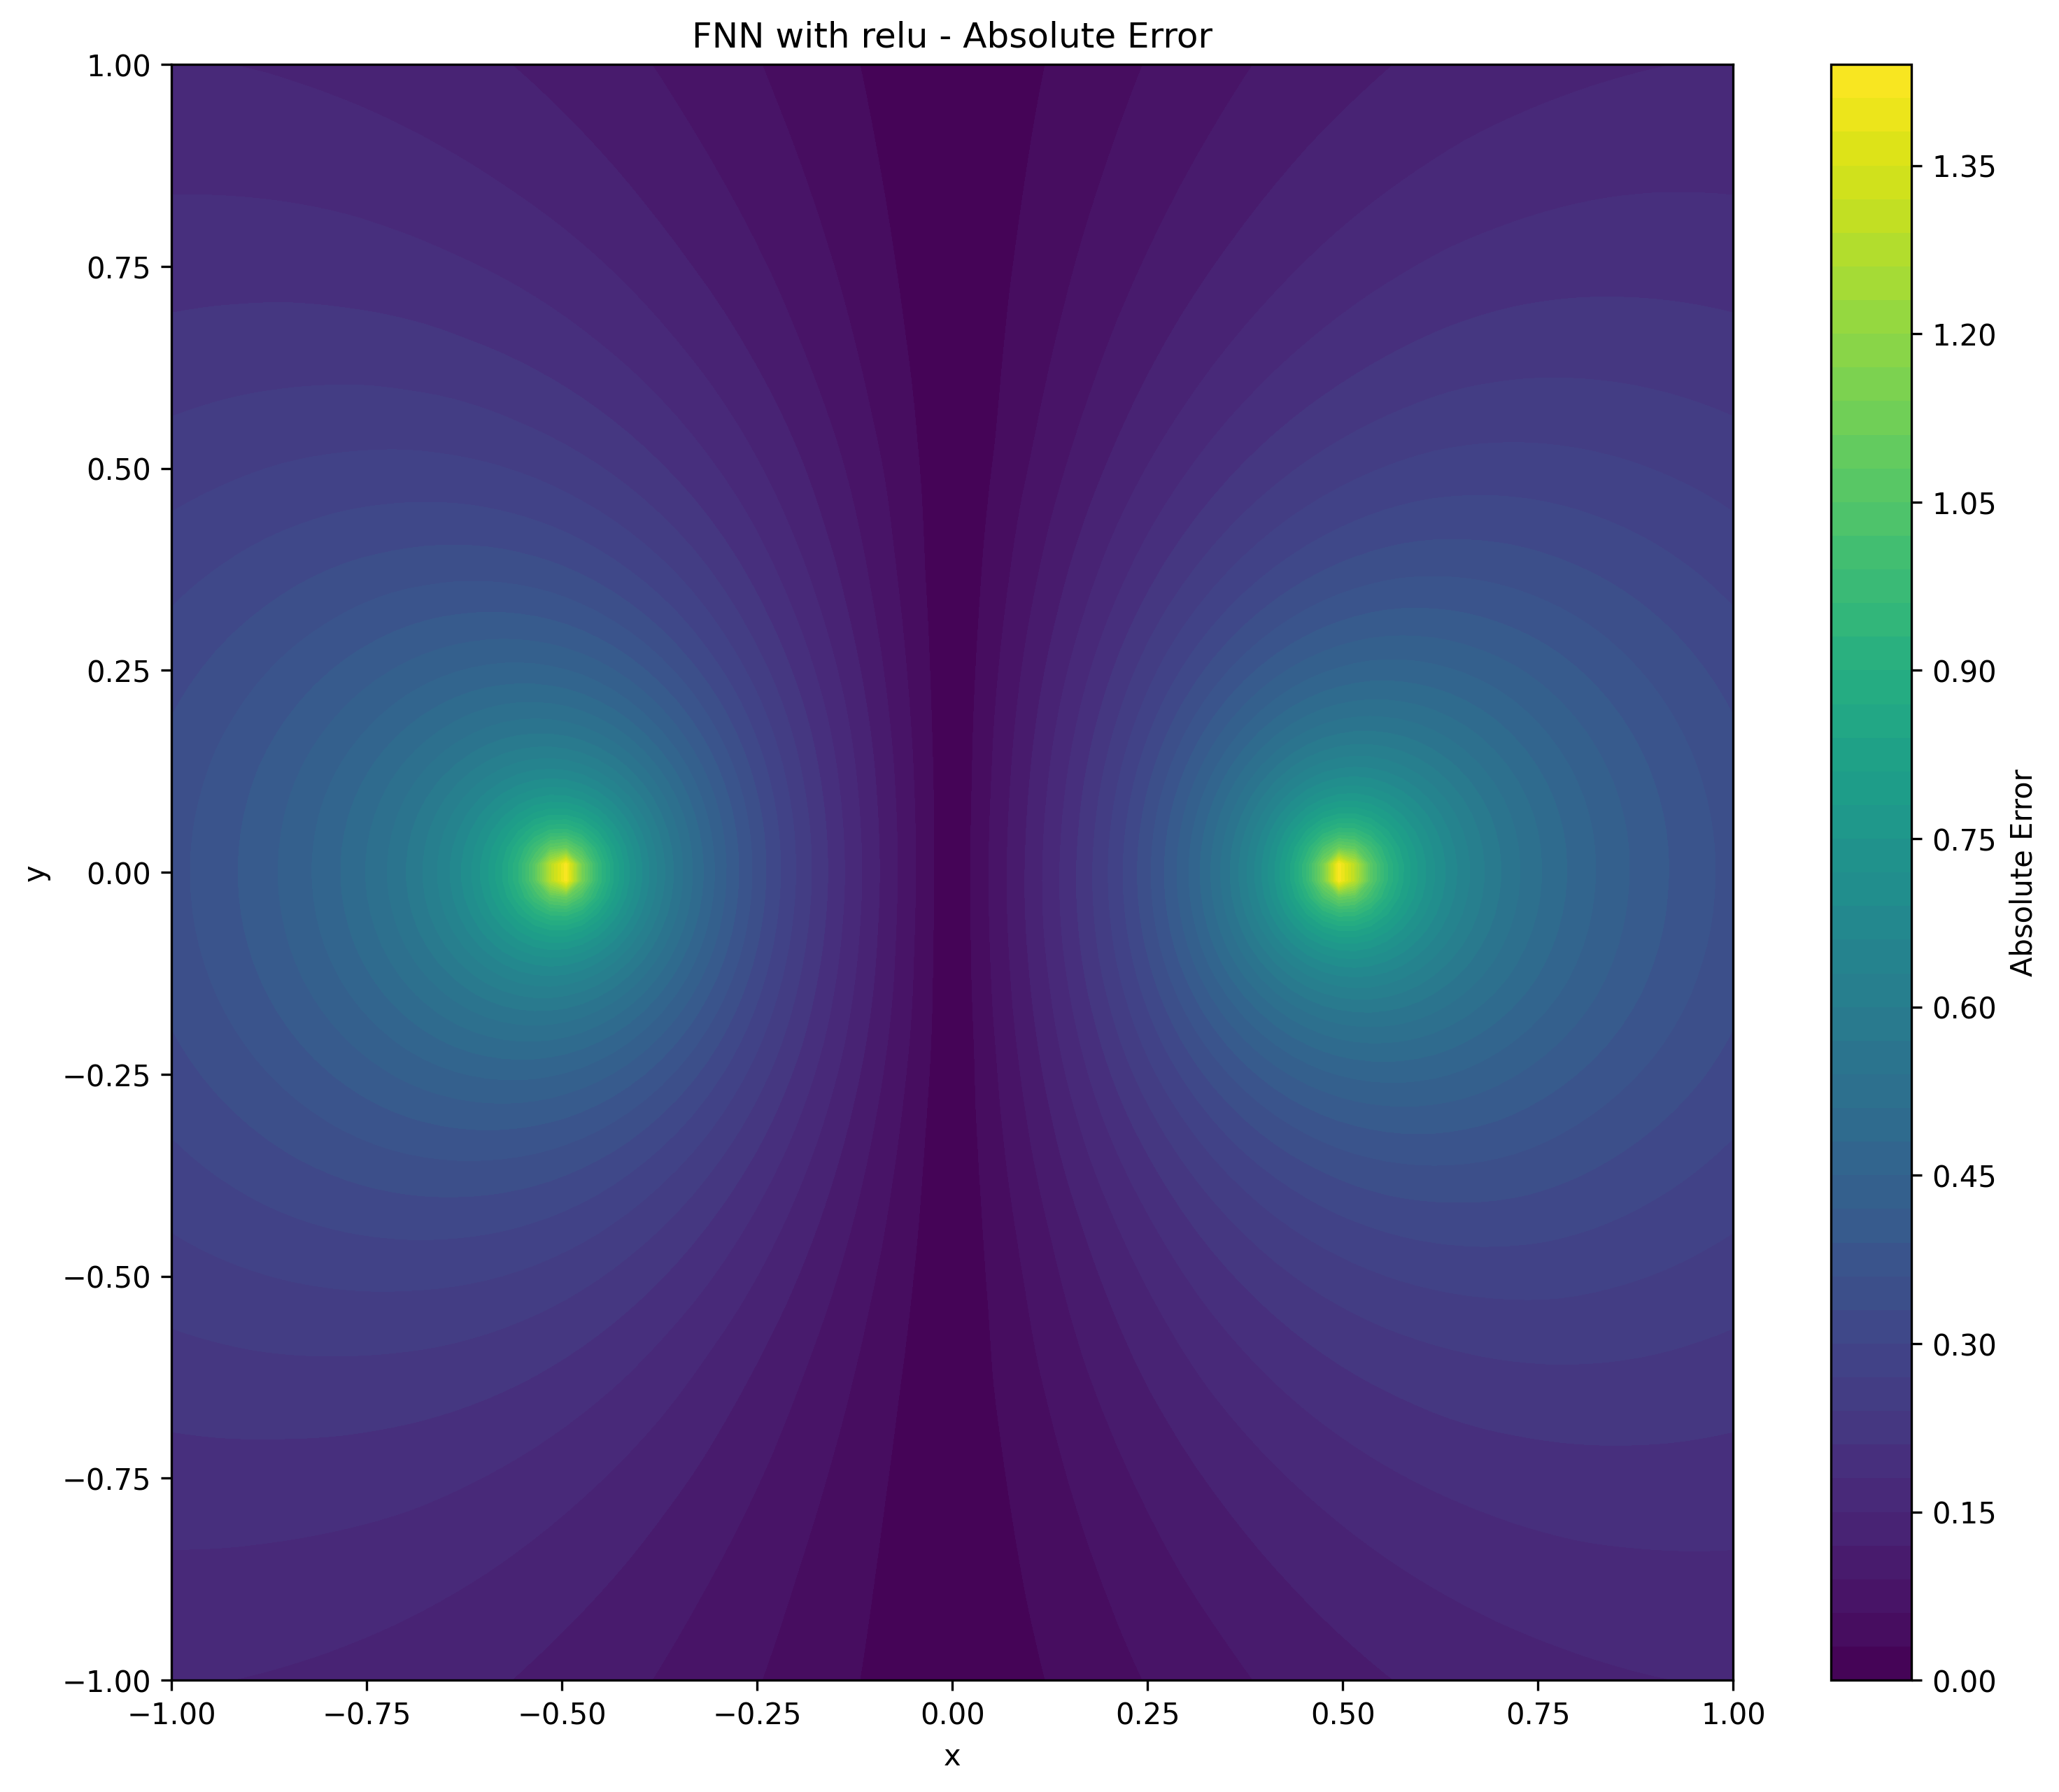
\includegraphics[width=\textwidth]{absolute_error.png}
			\caption{Absolute error for FNN with tanh}
		\end{subfigure}
		\caption{Solution and error visualization for the FNN architecture with tanh activation}
		\label{fig:architecture_solution}
	\end{figure}
	
	\section{Key Findings}
	
	From our experimental results, we can draw the following conclusions:
	
	\begin{itemize}
		\item \textbf{Architecture Impact}: Both FNN and ResNet architectures achieved similar accuracy levels (RMSE $\approx$ 0.294), while MsFFN maintained comparable accuracy but at a significantly higher computational cost. This aligns with findings from previous studies on architecture comparisons for PDEs \cite{chen2020comparison}.
		
		\item \textbf{Activation Functions}: The choice of activation function had a minimal impact on the final solution accuracy. However, some differences were observed in:
		\begin{itemize}
			\item \textbf{Training Efficiency}: ReLU activation resulted in the fastest training time (92.64s).
			\item \textbf{Final Loss}: Swish activation achieved the lowest final loss (6.98e-12).
		\end{itemize}
		Recent work by Jagtap et al. \cite{jagtap2020adaptive} confirms that adaptive activation functions can accelerate convergence in PINNs.
		
		\item \textbf{Error Distribution}: All models showed similar error patterns, with the highest errors concentrated near the point charges, where the singularities occur. This is a common challenge when dealing with singular Poisson problems \cite{huang2022solving}.
		
		\item \textbf{Best Overall Model}: The FNN with swish activation provided the best balance between accuracy and final loss, though at the cost of increased training time compared to FNN with ReLU.
	\end{itemize}
	
	These findings suggest that for the 2D Poisson equation with point singularities, simpler architectures like FNN with appropriate activation functions can achieve results comparable to more complex architectures while requiring significantly less computational resources \cite{wang2021understanding}. 
	\chapter{Conclusion and Future Work}
	
	\section{Conclusion}
	This project successfully implemented a Physics-Informed Neural Network to solve the 2D Poisson equation with point charge singularities \cite{huang2022solving}. The PINN approach showed good accuracy throughout the domain, with the expected higher errors near the singularities. The various visualization techniques provided comprehensive insights into the electric potential and field distributions.
	
	The key advantages of the PINN approach for this problem include:
	\begin{itemize}
		\item Ability to handle singularities through smooth approximations
		\item Mesh-free solution without the need for complex grid generation
		\item Good accuracy across the domain
		\item Rich visualization capabilities
	\end{itemize}
	
	\section{Future Work}
	Several avenues for future work include:
	\begin{enumerate}
		\item \textbf{Adaptive Sampling}: Implementing adaptive sampling techniques to focus more training points near the singularities \cite{meng2020ppinn}.
		\item \textbf{Extension to 3D}: Extending the approach to 3D problems, which are more relevant for many real-world applications.
		\item \textbf{Handling More Complex Charge Distributions}: Investigating more complex charge distributions and geometries \cite{gao2021phygeonet}.
		\item \textbf{Improved Network Architectures}: Exploring more advanced network architectures, such as residual networks or attention mechanisms \cite{jagtap2020conservative}.
		\item \textbf{Time-Dependent Problems}: Extending the approach to time-dependent problems, such as wave equations or heat equations \cite{meng2020ppinn}.
		\item \textbf{Multi-Physics Coupling}: Coupling the electrostatic problem with other physics, such as fluid dynamics or structural mechanics.
		\item \textbf{Uncertainty Quantification}: Incorporating uncertainty quantification into the PINN framework.
	\end{enumerate}
	
	These extensions would further enhance the capabilities and applicability of the PINN approach for solving complex PDE problems with singularities.
	
	\bibliography{references}
	\bibliographystyle{plain}
	
\end{document}